% ---- hand chunk 00-preamble.tex ----
\documentclass[11pt,a4paper,oneside,openany]{book}
% Thue--Morse Diagonal Laws: consolidated volume assembled 2026-09-05 from the
% three diagonal-polynomial arrivals of the 2026-09-03 intake; see the
% provenance appendix and README.md.
\usepackage[T1]{fontenc}
\usepackage[utf8]{inputenc}
\IfFileExists{libertinus.sty}{\usepackage{libertinus}}{\usepackage{lmodern}}
\usepackage{microtype}
\usepackage[a4paper,margin=26mm,headheight=15pt]{geometry}
\usepackage{amsmath,amssymb,amsthm,mathtools,bm}
\usepackage{booktabs,longtable,array,tabularx,multirow}
\usepackage[table]{xcolor}
\usepackage{tikz}
\usepackage{graphicx,enumitem,fancyhdr,listings,xurl}
\usepackage[hypertexnames=false]{hyperref}
\usepackage[nameinlink,noabbrev,capitalise]{cleveref}
% Canonical mathematical notation for active FabiusFunction LaTeX documents.
%
% This file is intentionally a plain TeX input rather than a LaTeX package.
% Every standalone document loads it by an explicit path relative to that
% document's directory; included fragments inherit the definitions from their
% root document.  Keep this file independent of document layout and metadata.
%
% Contract:
%   * one command has one mathematical meaning throughout the active corpus;
%   * names encode semantic roles rather than a document-local choice of letter;
%   * visually similar but differently normalized objects have different print;
%   * every command below is defined normatively in the notation catalogue.
%
% The active corpus excludes docs/archive/.  Historical sources may retain
% their original notation only inside an explicitly labelled quotation.

\makeatletter
\@ifundefined{mathbb}{%
  \PackageError{fabius-notation}{The amssymb package must be loaded first}%
    {Load amsmath and amssymb before inputting fabius-notation.tex.}%
}{}
\@ifundefined{operatorname}{%
  \PackageError{fabius-notation}{The amsmath package must be loaded first}%
    {Load amsmath before inputting fabius-notation.tex.}%
}{}
\makeatother

% Version stamp used by the catalogue and by static audits.
\newcommand{\FabiusNotationVersion}{2026-08-31}

% Number systems.  NaturalNumbers is explicitly the nonnegative convention.
\newcommand{\NaturalNumbers}{\mathbb{N}_{0}}
\newcommand{\PositiveIntegers}{\mathbb{N}_{>0}}
\newcommand{\IntegerNumbers}{\mathbb{Z}}
\newcommand{\RationalNumbers}{\mathbb{Q}}
\newcommand{\RealNumbers}{\mathbb{R}}
\newcommand{\ComplexNumbers}{\mathbb{C}}
\newcommand{\ExtendedRealNumbers}{\overline{\mathbb{R}}}

% The three principal Fabius--Rvachev functions.  Subscripts are deliberate:
% a bare F and a calligraphic F have several unrelated uses in the corpus.
\newcommand{\FabiusBounded}{F_{\mathrm{bd}}}
\newcommand{\FabiusGlobal}{F_{\mathrm{gl}}}
\newcommand{\FabiusQuantile}{Q_{F}}
\newcommand{\FabiusClampedQuantile}{Q_{F,\mathrm{cl}}}
\newcommand{\RvachevUp}{\operatorname{up}}

% Constants, elementary operators, and delimiters.
\newcommand{\EulerE}{\mathrm{e}}
\newcommand{\ImaginaryUnit}{\mathrm{i}}
\newcommand{\Differential}{\mathop{}\!\mathrm{d}}
\newcommand{\AbsoluteValue}[1]{\left\lvert #1\right\rvert}
\newcommand{\Norm}[1]{\left\lVert #1\right\rVert}
\newcommand{\Floor}[1]{\left\lfloor #1\right\rfloor}
\newcommand{\Ceiling}[1]{\left\lceil #1\right\rceil}
\newcommand{\FractionalPart}[1]{\left\{#1\right\}}
\newcommand{\PositivePart}[1]{\left(#1\right)_{+}}
\newcommand{\IndicatorOf}[1]{\mathbf{1}_{#1}}
\newcommand{\SetOf}[1]{\left\{#1\right\}}
\newcommand{\InnerProduct}[1]{\left\langle #1\right\rangle}
\newcommand{\CardinalityOf}[1]{\left\lvert #1\right\rvert}
\newcommand{\DefinitionEquals}{\mathrel{\coloneqq}}
\newcommand{\Sign}{\operatorname{sgn}}
\newcommand{\IdentityOperator}{\operatorname{id}}
\newcommand{\SpanOperator}{\operatorname{span}}
\newcommand{\TraceOperator}{\operatorname{tr}}
\newcommand{\RankOperator}{\operatorname{rank}}
\newcommand{\DiagonalOperator}{\operatorname{diag}}
\newcommand{\ResidueOperator}{\operatorname*{Res}}
\newcommand{\LeastCommonMultiple}{\operatorname{lcm}}
\newcommand{\OrderOperator}{\operatorname{ord}}
\newcommand{\PrincipalLogarithm}{\operatorname{Log}}
\newcommand{\FallingFactorial}[2]{\left(#1\right)^{\underline{#2}}}
\newcommand{\RisingFactorial}[2]{\left(#1\right)^{\overline{#2}}}

% Support, topology, convolution, and metric notation.
\newcommand{\SupportOperator}{\operatorname{supp}}
\newcommand{\SupportOf}[1]{\SupportOperator\!\left(#1\right)}
\newcommand{\TopologicalSupportOf}[1]{\operatorname{tsupp}\!\left(#1\right)}
\newcommand{\Convolution}{\mathbin{*}}
\newcommand{\MetricDistance}{\operatorname{dist}}
\newcommand{\TotalVariationDistance}{d_{\mathrm{TV}}}

% Probability.  Equality and convergence in law are not metric distance.
\newcommand{\Probability}{\mathbb{P}}
\newcommand{\Expectation}{\mathbb{E}}
\newcommand{\Variance}{\operatorname{Var}}
\newcommand{\Covariance}{\operatorname{Cov}}
\newcommand{\LawOperator}{\operatorname{Law}}
\newcommand{\LawOf}[1]{\LawOperator\!\left(#1\right)}
\newcommand{\EqualInLaw}{\mathrel{\overset{\mathrm{law}}{=}}}
\newcommand{\ConvergesInLaw}{\mathrel{\xrightarrow{\mathrm{law}}}}

% Fourier and integral transforms.  The printed labels expose normalization.
% FourierTwoPi uses exp(-2*pi*i*x*xi); FourierAngular uses exp(-i*x*omega).
\newcommand{\FourierTwoPi}[1]{\widehat{#1}_{\,2\pi}}
\newcommand{\FourierAngular}[1]{\widehat{#1}_{\,\mathrm{ang}}}
\newcommand{\LaplaceTransformSymbol}{\mathcal{L}}
\newcommand{\MellinTransformSymbol}{\mathcal{M}}
\newcommand{\LaplaceTransformOf}[1]{\LaplaceTransformSymbol\!\left[#1\right]}
\newcommand{\MellinTransformOf}[1]{\MellinTransformSymbol\!\left[#1\right]}
\newcommand{\MomentGeneratingFunction}[1]{M_{#1}}
\newcommand{\CharacteristicFunction}[1]{\varphi_{#1}}

% The two standard sinc functions must never share one symbol.
\newcommand{\SincRad}{\operatorname{sinc}_{\mathrm{rad}}}
\newcommand{\SincPi}{\operatorname{sinc}_{\pi}}

% Binary arithmetic and Thue--Morse notation.
\newcommand{\BinaryDigitSum}{\operatorname{wt}_{2}}
\newcommand{\ThueMorseSignSymbol}{\varepsilon}
\newcommand{\ThueMorseSign}[1]{\varepsilon_{#1}}
\newcommand{\PadicValuation}[1]{\nu_{#1}}
\newcommand{\TwoAdicValuation}{\nu_{2}}

% q-series notation.  Every base is an explicit argument.
\newcommand{\QPochhammer}[3]{\left(#1;#2\right)_{#3}}
\newcommand{\GaussianBinomial}[3]{%
  \genfrac{[}{]}{0pt}{}{#1}{#2}_{#3}%
}
\newcommand{\QInteger}[2]{\left[#1\right]_{#2}}

% Named special functions.
\newcommand{\Polylogarithm}{\operatorname{Li}}
\newcommand{\LambertW}{W}
\newcommand{\GammaFunction}{\Gamma}
\newcommand{\RiemannZeta}{\zeta}

% Asymptotics.  BigO and LittleO are operator tokens for existing formula
% grammar; prefer the At forms so that the limiting regime is printed.
\newcommand{\BigO}{\mathcal{O}}
\newcommand{\LittleO}{o}
\newcommand{\BigOAt}[2]{\mathcal{O}_{#2}\!\left(#1\right)}
\newcommand{\LittleOAt}[2]{o_{#2}\!\left(#1\right)}

\definecolor{linkblue}{RGB}{25,75,135}
\definecolor{shadegray}{RGB}{246,247,249}
\definecolor{rulegray}{RGB}{195,201,208}
\definecolor{rootcell}{RGB}{78,111,86}
\definecolor{lightroot}{RGB}{225,232,222}
\definecolor{codecomment}{RGB}{70,110,70}
\definecolor{codekeyword}{RGB}{40,60,150}
\hypersetup{colorlinks=true,linkcolor=linkblue,citecolor=linkblue,urlcolor=linkblue,
 pdftitle={Thue-Morse Diagonal Laws: Diagonal Polynomials and Dyadic Block Geometry in Repeated Thue-Morse Summation},
 pdfauthor={Consolidated volume for the ProveIt Fabius-function corpus},
 pdfsubject={Thue-Morse prefix sums, diagonal polynomials, Riordan arrays, Sheffer sequences, 2-adic Bell recurrences, half-integer roots, dyadic block geometry, fast exact evaluation}}
\allowdisplaybreaks
\raggedbottom
\setlength{\emergencystretch}{3em}
\setcounter{secnumdepth}{2}
\setcounter{tocdepth}{1}
\setlist[itemize]{leftmargin=2em,itemsep=0.25em,topsep=0.4em}
\setlist[enumerate]{leftmargin=2.4em,itemsep=0.25em,topsep=0.4em}
\pagestyle{fancy}
\fancyhf{}
\fancyhead[L]{\small\nouppercase{\leftmark}}
\fancyhead[R]{\small\thepage}
\renewcommand{\headrulewidth}{0.4pt}
\renewcommand{\chaptermark}[1]{\markboth{\thechapter.\ #1}{}}
\fancypagestyle{plain}{\fancyhf{}\fancyfoot[C]{\thepage}\renewcommand{\headrulewidth}{0pt}}
\numberwithin{equation}{chapter}
\newtheorem{theorem}{Theorem}[chapter]
\newtheorem{proposition}[theorem]{Proposition}
\newtheorem{corollary}[theorem]{Corollary}
\newtheorem{lemma}[theorem]{Lemma}
\newtheorem{conjecture}[theorem]{Conjecture}
\theoremstyle{definition}
\newtheorem{definition}[theorem]{Definition}
\newtheorem{algorithm}[theorem]{Algorithm}
\newtheorem{example}[theorem]{Example}
\theoremstyle{remark}
\newtheorem{remark}[theorem]{Remark}
\newtheorem{warning}[theorem]{Warning}
% ---- notation (the first report's letters; the others are mapped onto them) ----
\newcommand{\N}{\mathbb N}
\newcommand{\Nzero}{\mathbb N_0}
\newcommand{\Z}{\mathbb Z}
\newcommand{\Q}{\mathbb Q}
\newcommand{\R}{\mathbb R}
\newcommand{\eps}{\varepsilon}
\newcommand{\TM}{E}
\newcommand{\K}{E}
\newcommand{\wt}{s_2}
\newcommand{\bitsum}{s_2}
\newcommand{\coeff}[2]{[z^{#1}]\,#2}
\newcommand{\rising}[2]{#1^{\overline{#2}}}
\newcommand{\falling}[2]{#1^{\underline{#2}}}
\newcommand{\nuTwo}{\nu_2}
\newcommand{\vtwo}{\nu_2}
\newcommand{\vTwo}{\nu_2}
\newcommand{\bigO}{\mathcal O}
\newcommand{\Diag}{D}
\newcommand{\Dprim}{\widetilde D}
\newcommand{\Prefix}{T}
\newcommand{\PrefixOp}{\mathcal P}
\newcommand{\Bell}{\mathcal B}
\newcommand{\stirlingfirst}[2]{\genfrac{[}{]}{0pt}{}{#1}{#2}}
\newcommand{\stirlingone}[2]{\genfrac{[}{]}{0pt}{}{#1}{#2}}
\newcommand{\dd}{\,\mathrm d}
\newcommand{\ind}{\mathbf 1}
\newcommand{\Sgen}{\mathcal S}
\newcommand{\A}{Q}
\newcommand{\cont}{\operatorname{cont}}
\newcommand{\Up}{\operatorname{up}}
\DeclareMathOperator{\popcount}{popcount}
\DeclareMathOperator{\ord}{ord}
\DeclareMathOperator{\lcm}{lcm}
\DeclareMathOperator{\sgn}{sgn}
\newenvironment{boxedsummary}{%
  \par\medskip\noindent\begin{center}\begin{minipage}{0.94\textwidth}%
  \hrule\vspace{0.7em}\small
}{%
  \vspace{0.7em}\hrule\end{minipage}\end{center}\medskip
}
\newenvironment{resultbox}{%
  \par\smallskip\noindent\begin{center}\begin{minipage}{0.94\textwidth}%
  \color{black}\hrule\vspace{0.65em}\small
}{%
  \vspace{0.65em}\hrule\end{minipage}\end{center}\smallskip
}
\lstdefinelanguage{Wolfram}{
  morekeywords={ClearAll,Module,With,If,And,Table,Sum,Product,Expand,Factor,FullSimplify,
    Binomial,Factorial,Floor,Quotient,QuotientRemainder,Mod,IntegerExponent,IntegerLength,
    ThueMorse,Accumulate,Nest,CoefficientList,SeriesCoefficient,Coefficient,PossibleZeroQ,
    Take,Together,Numerator,Denominator,ConstantArray,OddQ,EvenQ,Range,Length,Select,Times,
    Flatten,MapThread,Total,HoldForm,SetDelayed,True,False},
  sensitive=true,
  morecomment=[s]{(*}{*)},
  morestring=[b]"
}
\lstdefinestyle{code}{
  basicstyle=\ttfamily\small,
  keywordstyle=\color{codekeyword}\bfseries,
  commentstyle=\color{codecomment},
  backgroundcolor=\color{shadegray},
  frame=single,
  rulecolor=\color{rulegray},
  columns=fullflexible,
  keepspaces=true,
  showstringspaces=false,
  breaklines=true,
  xleftmargin=0.6em,
  xrightmargin=0.6em,
  aboveskip=0.8em,
  belowskip=0.8em
}
\lstset{style=code}
\title{\Huge\bfseries Thue--Morse Diagonal Laws\\[4mm]
 \Large Diagonal Polynomials and Dyadic Block Geometry\\
 in Repeated Thue--Morse Summation\\[7mm]
 \large A consolidated volume for the Fabius-function corpus}
\author{Consolidated from three research reports with detailed proofs}
\date{September 5, 2026}

% ---- hand chunk 01-front.tex ----
\begin{document}
\frontmatter
\hypersetup{pageanchor=false}
\maketitle
\hypersetup{pageanchor=true}
\chapter*{Abstract}
\addcontentsline{toc}{chapter}{Abstract}
Consider the two-dimensional table specified by the signed Thue--Morse
prefix row and the weighted recurrence
\[
 s_{n,k}=\sum_{j=0}^{k-1}(k-j)s_{n-1,j}.
\]
Its first visible diagonals are polynomial in the row index, and the
originating program listed eight such laws. This volume derives the
polynomial on every diagonal and everything the three reports it
consolidates could say about it. Row $n$ is the $(2n+1)$-fold inclusive
prefix sum of the signed sequence shifted by $n+1$ columns; with
$r=k-n-1\ge0$,
\[
 s_{n,n+1+r}=\Diag_r(n),\qquad
 \Diag_r(x)=\sum_{q=0}^{\lfloor r/2\rfloor}\eps_q\binom{2x+r-2q-1}{r-2q},
 \qquad
 \sum_{r\ge0}\Diag_r(x)z^r=\frac{E(z^2)}{(1-z)^{2x}},
\]
where $E(z)=\prod_{j\ge0}(1-z^{2^j})=\sum\eps_qz^q$. Thus $\Diag_r$ has exact
degree $r$ and leading coefficient $2^r/r!$, all its monomial coefficients
are unsigned-Stirling sums, and the shifted table is the proper Riordan
array $(E(z^2),z/(1-z)^2)$; a general subdiagonal theorem for proper Riordan
arrays explains the polynomiality. The logarithm of the diagonal generating
function has the $2$-adic cumulants $\lambda_m(x)=2x+2-2^{\nu_2(m)+1}$, so the
polynomials obey a Newton--Bell recurrence, partition and determinant
formulas, a Sheffer half-step lowering law
$\Diag_r(x)-\Diag_r(x-\tfrac12)=\Diag_{r-1}(x)$, translation, differential
and addition laws, and a binary Mahler self-similarity. The arithmetic is
exact: $r!\Diag_r(x)/2^{\lceil r/2\rceil}$ is a primitive integer polynomial,
which gives the exact common denominator of every diagonal, and every
rational zero is an integer or a half-integer. All nonnegative rational
zeros are classified by a dyadic residue condition, negative half-grid
values are finite backward differences of the signed sequence, and an
infinite family of negative integer roots is proved.

For each fixed row the entire sequence is a signed repetition of one
nonnegative block of length $2^{2n+1}$; the volume proves its support,
circular reflection, complement law, exact central plateau, maximum, mass,
moments, multiplicities and number of distinct values, and the finite-block
theorem for every order of iterated summation from which these follow. The
block coefficients are the level-$2n$ Rvachev histogram of the corpus, and
suitably scaled rows converge to the up-function and the Fabius function.
Exact algorithms are given for every regime: symbolic generation of any
diagonal, direct evaluation near the edge, signed-block reduction, and a
logarithmic-time evaluator through signed Thue--Morse prefix moments. The
three exact verification programs and Wolfram Language implementations
shipped with the sources are retained.

\chapter*{Relation to the atlas and to the three sources}
\addcontentsline{toc}{chapter}{Relation to the atlas and to the three sources}
The atlas \cite{atlas} proves the exact prefix collapse, the iterated-prefix
convolution and generating function, terminal dyadic zero runs, and signed
reversal, with Lean crosswalks for those statements; the repository's Lean
development also formalizes the finite approximation polynomials, the
corrected normalization, and the step approximants
\cite{proveit-prefix,proveit-approx}. Those facts are inputs here. The
volume's own contribution is the reorganization around the two indices
$(n,k)$ and the complete fixed-diagonal polynomial calculus.

\paragraph{The three sources.}
This volume replaces three independently written reports on the same
table, filed together on September 3, 2026: a proof-oriented note
organized around the diagonal coordinate, Sheffer and ruler recurrences,
half-integer roots and the finite-block geometry of every summation order;
a report emphasizing the Riordan-array structure, $2$-adic Newton--Bell
recurrences, primitive normalization and exact denominators, the
rational-root restriction, and a fast prefix-moment evaluator; and a report
emphasizing the pulse polynomial of every row, the exact content of doubled
rising factorials, the diagonal Mahler equation, the half-grid
transposition, a provable family of negative integer roots, and the exact
identification of the rows with the Rvachev histogram approximants. All
three proved the same core (the table identification, the row and bivariate
generating functions, the sparse rising-factorial formula, the monomial
coefficients, the half-step, differential and addition laws, the
$2$-adic recurrence, the nonnegative half-integer root criterion, the
negative half-grid formula, and the finite-block factorization). Each such
result is stated once, in the form that carried the most complete proof,
and the two other reports' variant formulations are kept only where they
add a formula. The first report's notation is used throughout; the
provenance appendix records the dictionary. Statements imported verbatim
from the second and third reports write the diagonal index as $m$ and $q$
respectively where the first writes $r$; the polynomial is the same
$\Diag$.

The volume loads the corpus notation file \path{docs/fabius-notation.tex}
for consistency with the other volumes. No Lean formalization is claimed
for any result here; the closing chapter lists the formalization targets.
\begingroup
\small
\tableofcontents
\endgroup

\mainmatter

% ---- A lines 148--224 ----
\chapter{Problem, conventions, and main answer}\label{ch:problem}

\section{The table}

Let
\begin{equation}
  \eps_q=(-1)^{\wt(q)},\qquad q\in\Nzero,
  \label{a:eq:tm-sign}
\end{equation}
where \(\wt(q)\) is the number of ones in the binary expansion of \(q\).
This is the signed Thue--Morse sequence.  Throughout the volume, \(n\) and
\(k\) are nonnegative integers.  The originating program is read as defining
\(s_{n,k}\) with the triangular initial condition \(s_{n,k}=0\) for
\(k\le n\), the signed-prefix row at \(n=0\), and the fallback recurrence
\begin{equation}
  s_{n,k}=\sum_{j=0}^{k-1}(k-j)s_{n-1,j},\qquad n\ge1.
  \label{a:eq:weighted-recurrence}
\end{equation}
The symmetry branches and the first eight diagonal formulas are computational
shortcuts.  We will derive them rather than assume them.

The repository's Thue--Morse atlas proves the exact prefix collapse, the
iterated-prefix convolution and generating function, terminal dyadic zero
runs, and signed reversal, with explicit Lean crosswalks for those statements
\cite{atlas}.  The present volume reorganizes those ingredients around
the two indices \((n,k)\), and develops the fixed-diagonal polynomial calculus.
No priority claim is made for identities that follow from standard formal
power-series manipulations.

\section{The diagonal coordinate}

The first nonzero entry of row \(n\) occurs at \(k=n+1\).  It is therefore
natural to set
\begin{equation}
  r=k-n-1.
  \label{a:eq:r-coordinate}
\end{equation}
The visible diagonal \(k-n=d\) in the original table corresponds to
\(r=d-1\).  We reserve \(\Diag_r(x)\) for the polynomial attached to this
offset.

\begin{boxedsummary}
\textbf{Closed form for an arbitrary diagonal.}
For every \(r\ge0\), define
\begin{equation}
 \boxed{
 \Diag_r(x)=
 \sum_{q=0}^{\lfloor r/2\rfloor}
 \eps_q\binom{2x+r-2q-1}{r-2q}
 =\sum_{q=0}^{\lfloor r/2\rfloor}
 \eps_q\frac{\rising{2x}{r-2q}}{(r-2q)!}.}
 \label{a:eq:main-diagonal}
\end{equation}
Then
\begin{equation}
 \boxed{
 s_{n,k}=\begin{cases}
 0,&k\le n,\\[2mm]
 \Diag_{k-n-1}(n),&k\ge n+1.
 \end{cases}}
 \label{a:eq:main-table-answer}
\end{equation}
Equivalently, the polynomial on the original diagonal \(d=k-n\ge1\) is
\begin{equation}
 \boxed{
 P_d(x)=\Diag_{d-1}(x)=
 \sum_{q=0}^{\lfloor(d-1)/2\rfloor}
 \eps_q\binom{2x+d-2q-2}{d-2q-1}.}
 \label{a:eq:main-d-answer}
\end{equation}
It has degree \(d-1\) and leading coefficient \(2^{d-1}/(d-1)!\).
\end{boxedsummary}

Formula \eqref{a:eq:main-diagonal} is finite and exact.  It is not an
interpolation guessed from numerical rows: it follows coefficientwise from a
single generating function, and hence applies to every row and every
nonnegative column.
% ---- B lines 232--242 ----
\begin{resultbox}
\textbf{Indexing guide.}
The row parameter $n$ in the code is not the number of prefix summations.
Row $n$ contains the $(2n+1)$-fold inclusive prefix sum, shifted right by
$n+1$ columns.  The natural diagonal coordinate is
\[
 m=k-n-1.
\]
The polynomial $\Diag_m(x)$ describes the line $k=n+1+m$; its value at the
integer $x=n$ is exactly the table entry on that line.
\end{resultbox}
% ---- hand chunk 02-summary.tex ----

\section{Summary of the structural results}

Beyond the closed form, the volume proves the following.

\begin{enumerate}
\item The row generating function is
\[
 A_n(z):=\sum_{k\ge0}s_{n,k}z^k
 =\frac{z^{n+1}E(z^2)}{(1-z)^{2n}}
 =\frac{z^{n+1}E(z)}{(1-z)^{2n+1}},
\]
so the shifted row is exactly an odd-order iterated prefix,
$s_{n,n+1+r}=\Prefix_r^{(2n+1)}$, and the shifted table is the proper Riordan
array $(E(z^2),z/(1-z)^2)$ (\cref{ch:riordan}). Every proper Riordan array
has polynomial subdiagonals; here the degree is exactly $r$.

\item The sequence $\widehat\Diag_r(x)=r!\Diag_r(x)$ is Sheffer for
$E(z^2)\exp(-2x\log(1-z))$. In particular
\[
 \Diag_r(x)-\Diag_r(x-\tfrac12)=\Diag_{r-1}(x),
 \qquad
 r\Diag_r(x)=\sum_{m=1}^r\bigl(2x+2-2^{\nuTwo(m)+1}\bigr)\Diag_{r-m}(x),
\]
with Bell, partition and determinant forms of the second identity,
translation, differential and addition laws, and the binary self-similarity
$G_x(z)=(1-z)(1+z)^{2x+1}G_x(z^2)$ of the generating function
(\cref{ch:sheffer}).

\item $r!\Diag_r(x)/2^{\lceil r/2\rceil}$ is a primitive integer polynomial,
the exact common denominator of $\Diag_r$ is
$r!/2^{\min(\nuTwo(r!),\lceil r/2\rceil)}$, and every rational zero of
$\Diag_r$ lies in $\tfrac12\Z$ (\cref{ch:arithmetic}).

\item For $m\ge0$,
\[
 \Diag_r(m/2)=0
 \iff
 r\bmod 2^{m+1}\in\{2^{m+1}-(m+1),\ldots,2^{m+1}-1\},
\]
and $\Diag_r(m/2)=\Prefix_r^{(m+1)}$ reads a fixed column vertically through
all prefix orders; negative half-integer values are finite backward
differences of the signed sequence, and $\Diag_r(-2^\ell)=0$ whenever
$r\equiv-1\pmod{2^a}$ and $\ell$ is odd with $\ell\le a-1$
(\cref{ch:roots}).

\item A row has block length $L=2^{2n+1}$, block maximum
$M_n=2^{\binom{2n}{2}}$, exactly $2n+1$ zero positions, exactly $2n+1$
maximum positions, and $2^{2n}-2n+1$ distinct absolute values; every
nonextreme value occurs exactly twice, the block is palindromic and
complement-symmetric, and its normalized coefficients are the probability
mass function of a sum of independent discrete uniforms
(\cref{ch:blocks,ch:rows}). Divided by $M_n$ they are the level-$2n$ Rvachev
histogram samples, and the rows converge to the up-function and the Fabius
function under the dyadic scaling (\cref{ch:fabius}).

\item Every table entry can be computed exactly in $O(n^2\log r)$ arithmetic
operations, where $r=k-n-1$, through a binary divide-and-conquer recurrence
for the signed prefix moments $\sum_{q<N}\eps_qq^d$ (\cref{ch:algorithms}).
\end{enumerate}

% ---- A lines 275--352 ----
\chapter{Signed Thue--Morse prefixes and formal products}\label{ch:prefixes}

\section{The lacunary product}

The binary recursions
\begin{equation}
  \eps_{2q}=\eps_q,
  \qquad
  \eps_{2q+1}=-\eps_q
  \label{a:eq:tm-recursion}
\end{equation}
imply the formal product identity
\begin{equation}
 E(z):=\sum_{q\ge0}\eps_qz^q
 =\prod_{j\ge0}(1-z^{2^j}).
 \label{a:eq:E-product}
\end{equation}
Every coefficient of the infinite product stabilizes after finitely many
factors, so \eqref{a:eq:E-product} is valid in \(\Z[[z]]\); no analytic
convergence is required.  Separating the first factor gives the Mahler
relation
\begin{equation}
 E(z)=(1-z)E(z^2).
 \label{a:eq:Mahler}
\end{equation}
These identities are standard in the theory of automatic sequences
\cite{allouche-shallit-book}; they are also the algebraic engine of the repository's
Fabius--Rvachev development \cite{atlas}.

\section{Exclusive and inclusive prefixes}

Define the exclusive prefix
\begin{equation}
 S(k)=\sum_{j=0}^{k-1}\eps_j,
 \qquad S(0)=0.
 \label{a:eq:exclusive-prefix}
\end{equation}
Pairing \(\eps_{2q}+\eps_{2q+1}=0\) gives
\begin{equation}
 S(2q)=0,
 \qquad
 S(2q+1)=\eps_q.
 \label{a:eq:prefix-collapse}
\end{equation}
Consequently,
\begin{equation}
 \sum_{k\ge0}S(k)z^k
 =zE(z^2)
 =\frac{zE(z)}{1-z}.
 \label{a:eq:prefix-gf}
\end{equation}
This is precisely the \(n=0\) row encoded by the supplied Wolfram Language
branches.

For comparison with repeated summation, define inclusive iterates
\begin{equation}
 \Prefix_r^{(0)}=\eps_r,
 \qquad
 \Prefix_r^{(h+1)}=\sum_{j=0}^{r}\Prefix_j^{(h)}.
 \label{a:eq:inclusive-prefix-definition}
\end{equation}
One summation multiplies an ordinary generating function by \((1-z)^{-1}\),
so
\begin{equation}
 \sum_{r\ge0}\Prefix_r^{(h)}z^r
 =\frac{E(z)}{(1-z)^h}.
 \label{a:eq:inclusive-prefix-gf}
\end{equation}
For \(h\ge1\), coefficient extraction yields
\begin{equation}
 \Prefix_r^{(h)}
 =\sum_{j=0}^{r}
 \binom{r-j+h-1}{h-1}\eps_j.
 \label{a:eq:inclusive-prefix-convolution}
\end{equation}
Bertazzon's construction of a solution to a Thue--Morse integral equation uses
these repeated sums and their dyadic block coefficients in essentially this
form \cite{bertazzon}.
% ---- A lines 354--421 ----
\chapter{Generating function of the complete two-dimensional table}\label{ch:table}

\section{The weighted recurrence as two summations}

Let
\begin{equation}
 A_n(z)=\sum_{k\ge0}s_{n,k}z^k.
 \label{a:eq:row-gf-definition}
\end{equation}
The kernel in \eqref{a:eq:weighted-recurrence} has generating function
\begin{equation}
 \sum_{m\ge1}m z^m=\frac{z}{(1-z)^2}.
 \label{a:eq:kernel-gf}
\end{equation}
Thus \eqref{a:eq:weighted-recurrence} is convolution by the coefficient sequence
\(1,2,3,\ldots\), or equivalently two discrete antiderivatives together with
a one-step shift.

\begin{theorem}[Exact row generating function]
For every \(n\ge0\),
\begin{equation}
 \boxed{
 A_n(z)=
 \left(\frac{z}{(1-z)^2}\right)^n zE(z^2)
 =\frac{z^{n+1}E(z^2)}{(1-z)^{2n}}
 =\frac{z^{n+1}E(z)}{(1-z)^{2n+1}}.}
 \label{a:eq:row-gf}
\end{equation}
\end{theorem}

\begin{proof}
Equation \eqref{a:eq:prefix-gf} gives \(A_0(z)=zE(z^2)\).  Multiplying by
\eqref{a:eq:kernel-gf} implements the recurrence once, so induction gives the
first two expressions.  The last follows from the Mahler identity
\eqref{a:eq:Mahler}.
\end{proof}

The triangular zero region is now automatic: \(A_n\) is divisible by
\(z^{n+1}\).  More importantly, shifting by this monomial identifies each row
with a standard iterated-prefix sequence.

\begin{corollary}[Rows are odd-order iterated prefixes]
For every \(n,r\ge0\),
\begin{equation}
 \boxed{s_{n,n+1+r}=\Prefix_r^{(2n+1)}.}
 \label{a:eq:row-prefix-identification}
\end{equation}
Equivalently,
\begin{equation}
 s_{n,n+1+r}
 =\sum_{j=0}^{r}\eps_j\binom{2n+r-j}{2n}.
 \label{a:eq:row-prefix-convolution}
\end{equation}
\end{corollary}

\begin{proof}
After removing \(z^{n+1}\) from \eqref{a:eq:row-gf}, the remaining generating
function is \(E(z)/(1-z)^{2n+1}\), which is
\eqref{a:eq:inclusive-prefix-gf} with \(h=2n+1\).
\end{proof}

This relation also identifies the absolute values in the earlier question on
periodic iterated Thue--Morse sums.  With the notation used there,
\begin{equation}
 |s_{n,n+1+r}|=u_r^{(2n)}.
 \label{a:eq:mathse-map}
\end{equation}
The row index \(n\) therefore advances the summation order by two.
% ---- hand chunk 11-ch3-rows-lead.tex ----

The first rows illustrate both the initial zero triangle and the rapid
formation of a positive pulse, which \cref{ch:rows} describes exactly.

% ---- C lines 368--381 ----
\begin{center}
\small
\setlength{\tabcolsep}{3.6pt}
\begin{tabular}{c|rrrrrrrrrrrrrrrrr}
\toprule
\(n\backslash k\)&0&1&2&3&4&5&6&7&8&9&10&11&12&13&14&15&16\\
\midrule
0&0&1&0&-1&0&-1&0&1&0&-1&0&1&0&1&0&-1&0\\
1&0&0&1&2&2&2&1&0&0&0&-1&-2&-2&-2&-1&0&0\\
2&0&0&0&1&4&9&16&24&32&40&48&55&60&63&64&64&64\\
3&0&0&0&0&1&6&20&50&104&190&316&490&719&1008&1360&1776&2256\\
\bottomrule
\end{tabular}
\end{center}
% ---- hand chunk 10-ch3-local-lead.tex ----

\section{A local discrete equation}
The row generating functions form a geometric sequence, which turns the
cumulative recurrence into a local second-difference law.

% ---- B lines 379--404 ----
In particular,
\begin{equation}
 \frac{A_n(z)}{A_{n-1}(z)}=\frac{z}{(1-z)^2}
 \qquad(n\ge1).
 \label{b:eq:row-ratio}
\end{equation}
The cumulative recurrence in the original code is therefore the integrated
form of a local second-difference law.

\begin{corollary}[Local discrete equation]
\label{b:cor:local-pde}
With the convention $s_{n,k}=0$ for $k<0$, one has, for $n\ge1$,
\begin{equation}
 s_{n,k}-2s_{n,k-1}+s_{n,k-2}=s_{n-1,k-1}.
 \label{b:eq:local-pde}
\end{equation}
\end{corollary}

\begin{proof}
Multiply \eqref{b:eq:row-ratio} by $(1-z)^2$ and compare coefficients of
$z^k$.
\end{proof}

Equation \eqref{b:eq:local-pde} fills a rectangular portion of the table in
constant work per cell.  It is often preferable to reevaluating the weighted
sum in \eqref{a:eq:weighted-recurrence} for each new cell.
% ---- A lines 423--454 ----
\section{Two bivariate generating functions}

Summing \eqref{a:eq:row-gf} over the row index gives a compact encoding of the
whole array.

\begin{proposition}[Bivariate table generating function]
As a formal power series in \(u\) with coefficients in \(\Z[[z]]\),
\begin{equation}
 \boxed{
 \sum_{n\ge0}\sum_{k\ge0}s_{n,k}u^nz^k
 =\frac{z(1-z)^2E(z^2)}{(1-z)^2-uz}.}
 \label{a:eq:bivariate-table}
\end{equation}
For the diagonal array \(\Diag_r(n)=s_{n,n+1+r}\),
\begin{equation}
 \boxed{
 \sum_{n\ge0}\sum_{r\ge0}\Diag_r(n)u^nz^r
 =\frac{(1-z)^2E(z^2)}{(1-z)^2-u}.}
 \label{a:eq:bivariate-diagonal}
\end{equation}
\end{proposition}

\begin{proof}
Both formulas are geometric sums.  For example,
\[
 \sum_{n\ge0}u^nA_n(z)
 =zE(z^2)\sum_{n\ge0}
 \left(\frac{uz}{(1-z)^2}\right)^n.
\]
Removing the shift \(z^{n+1}\) before summing gives
\eqref{a:eq:bivariate-diagonal}.
\end{proof}
% ---- A lines 456--558 ----
\chapter{Why fixed-index iterated sums are polynomials}\label{ch:polynomiality}

The polynomial phenomenon is not peculiar to Thue--Morse.  It is a universal
property of repeated summation, sharpened here by the Mahler factorization.

\section{A general summation-order polynomial}

Let \(a_0,a_1,\ldots\) be any sequence over a characteristic-zero field and
let
\[
 A(z)=\sum_{j\ge0}a_jz^j.
\]
For an integer \(h\ge0\), write \(U_r^{(h)}\) for the \(h\)-fold inclusive
sum, so its generating function is \(A(z)/(1-z)^h\).

\begin{theorem}[Polynomiality in the summation order]
For each fixed \(r\ge0\), the coefficient
\begin{equation}
 U_r(h):=\coeff{r}{\frac{A(z)}{(1-z)^h}}
 \label{a:eq:general-U}
\end{equation}
extends from \(h\in\Nzero\) to the polynomial
\begin{equation}
 \boxed{
 U_r(h)=\sum_{j=0}^{r}a_j
 \binom{h+r-j-1}{r-j}.}
 \label{a:eq:general-order-polynomial}
\end{equation}
Its degree is at most \(r\), and is exactly \(r\) if \(a_0\ne0\), with
leading coefficient \(a_0/r!\).
\end{theorem}

\begin{proof}
Expand
\[
 (1-z)^{-h}=\sum_{m\ge0}\binom{h+m-1}{m}z^m
\]
formally and take the Cauchy coefficient at \(z^r\).  For fixed \(m\), the
generalized binomial coefficient is a polynomial in \(h\) of degree \(m\).
Only the term \(j=0\), for which \(m=r\), can contribute degree \(r\).
\end{proof}

The value at \(h=0\) is included: the generalized binomial vanishes for
positive lower index and upper index one smaller, leaving \(U_r(0)=a_r\).
This polynomial continuation is therefore canonical, not an arbitrary fit.

\section{Mahler deflation and sparse diagonals}

Many automatic sequences have a functional factorization that compresses the
sum \eqref{a:eq:general-order-polynomial}.

\begin{theorem}[A general deflation principle]
Suppose
\begin{equation}
 A(z)=(1-z)^cB(z^b),
 \qquad
 B(z)=\sum_{q\ge0}b_qz^q,
 \label{a:eq:general-deflation-hypothesis}
\end{equation}
where \(b\ge2\) and \(c\in\Z\).  Then
\begin{equation}
 \boxed{
 U_r(h)=
 \sum_{q=0}^{\lfloor r/b\rfloor}b_q
 \binom{h-c+r-bq-1}{r-bq}.}
 \label{a:eq:general-deflation}
\end{equation}
Thus only one residue class modulo \(b\) of coefficient degrees occurs.
\end{theorem}

\begin{proof}
Substitute \eqref{a:eq:general-deflation-hypothesis} into
\eqref{a:eq:general-U}:
\[
 \frac{A(z)}{(1-z)^h}=B(z^b)(1-z)^{-(h-c)}.
\]
The term \(b_qz^{bq}\) leaves coefficient degree \(r-bq\) in the binomial
series.
\end{proof}

For Thue--Morse, \eqref{a:eq:Mahler} has \(b=2\), \(c=1\), and \(B=E\).
Therefore
\begin{equation}
 \Prefix_r^{(h)}
 =\sum_{q=0}^{\lfloor r/2\rfloor}
 \eps_q\binom{h+r-2q-2}{r-2q}.
 \label{a:eq:prefix-order-polynomial}
\end{equation}
Since the table uses \(h=2n+1\), formula \eqref{a:eq:main-diagonal} follows
immediately.  This proves the main answer \eqref{a:eq:main-table-answer}.

\begin{remark}[Interpretation]
For a fixed coefficient index \(r\), \(\Diag_r(x)\) is the polynomial
continuation of the \(h\)-fold signed Thue--Morse prefix under the affine
change \(h=2x+1\):
\begin{equation}
 \Diag_r(x)=\Prefix_r^{(2x+1)}
 \quad\text{in the sense of polynomial continuation in }h.
 \label{a:eq:polynomial-interpolation-interpretation}
\end{equation}
At integer \(x=n\), this is exactly the row identity
\eqref{a:eq:row-prefix-identification}.
\end{remark}
% ---- B lines 416--580 ----
\chapter{Riordan-array structure and a general subdiagonal theorem}
\label{b:sec:riordan}\label{ch:riordan}

\section{The shifted table is a proper Riordan array}

Shift the column index once and transpose the visual convention by setting
\begin{equation}
 A_{r,n}=s_{n,r+1},
 \qquad r,n\ge0.
 \label{b:eq:A-definition}
\end{equation}
Then $A_{r,n}=0$ for $r<n$ and $A_{n,n}=1$.  From
\eqref{a:eq:row-gf},
\begin{equation}
 A_{r,n}
 =\coeff{r}{\TM(z^2)\left(\frac{z}{(1-z)^2}\right)^n}.
 \label{b:eq:riordan-entry}
\end{equation}
Thus $A$ is the proper ordinary Riordan array
\begin{equation}
 A=\left(\TM(z^2),\frac{z}{(1-z)^2}\right).
 \label{b:eq:riordan-pair}
\end{equation}
We use the convention that a Riordan pair $(g,f)$ denotes the lower-triangular
matrix $[z^r]g(z)f(z)^n$.  Standard background can be found in
\cite{shapiro,sprugnoli}; all facts needed below are also proved
directly.

The compositional inverse of
$f(z)=z/(1-z)^2$ is
\begin{equation}
 \bar f(w)
 =\frac{1+2w-\sqrt{1+4w}}{2w}
 =\frac{\sqrt{1+4w}-1}{\sqrt{1+4w}+1}
 =w-2w^2+5w^3-14w^4+\cdots.
 \label{b:eq:f-inverse}
\end{equation}
Consequently the inverse unitriangular matrix is the Riordan array
\begin{equation}
 A^{-1}
 =\left(\frac{1}{\TM(\bar f(z)^2)},\bar f(z)\right).
 \label{b:eq:riordan-inverse}
\end{equation}
This inverse is not needed to generate the table, but it shows that the table
is an invertible change of basis over $\Z$: both $f$ and $\bar f$ have
integer coefficients and $\TM(0)=1$.

\section{Why fixed subdiagonals are always polynomials}

The polynomial phenomenon is not accidental and is not special to
Thue--Morse.  It is a general feature of proper Riordan arrays.

\begin{theorem}[Polynomial subdiagonals of a proper Riordan array]
\label{b:thm:general-riordan-diagonal}
Let $K$ be a characteristic-zero field, let
$g(z)\in K[[z]]$ satisfy $g(0)=g_0\ne0$, and let
$\phi(z)\in K[[z]]$ satisfy $\phi(0)=1$.  Form the proper Riordan array
\[
 R_{r,n}=\coeff{r}{g(z)\bigl(z\phi(z)\bigr)^n}.
\]
For every fixed $m\ge0$, define the formal continuation of the $m$th
subdiagonal by
\begin{equation}
 P_m(x)=\coeff{m}{g(z)\phi(z)^x},
 \qquad
 \phi(z)^x:=\exp\!\bigl(x\log\phi(z)\bigr).
 \label{b:eq:general-subdiagonal}
\end{equation}
Then:
\begin{enumerate}
 \item $P_m(x)\in K[x]$ and $\deg P_m\le m$;
 \item $P_m(n)=R_{n+m,n}$ for every $n\in\N$;
 \item if $\phi_1=[z]\phi(z)\ne0$, then $\deg P_m=m$ and
 \begin{equation}
  [x^m]P_m(x)=\frac{g_0\phi_1^m}{m!}.
  \label{b:eq:general-leading}
 \end{equation}
\end{enumerate}
\end{theorem}

\begin{proof}
Write $L(z)=\log\phi(z)$.  Since $\phi(0)=1$, one has
$L(z)\in zK[[z]]$.  Therefore
\[
 g(z)\phi(z)^x
 =g(z)\sum_{j\ge0}\frac{x^jL(z)^j}{j!}.
\]
Because $L(z)^j$ has order at least $j$, only $j\le m$ can contribute to
$[z^m]$.  This proves polynomiality and the degree bound.  At a
nonnegative integer $x=n$, the formal power $\phi(z)^x$ is the ordinary
$n$th power, so
\[
 P_m(n)=[z^m]g(z)\phi(z)^n
       =[z^{n+m}]g(z)(z\phi(z))^n
       =R_{n+m,n}.
\]
Finally, the coefficient of $x^m$ can only come from $j=m$.  To reach
$z^m$ in $g(z)L(z)^m$, one must take the constant $g_0$ and the linear term
$\phi_1z$ from every copy of $L$.  This gives
$g_0\phi_1^m/m!$.
\end{proof}

\begin{remark}
The theorem gives a canonical polynomial, not merely an interpolation through
integer points.  Formula \eqref{b:eq:general-subdiagonal} defines it in the
coefficient ring before any values are sampled.  This distinction matters
when one studies coefficients, denominators, roots, or values at half-integer
arguments.
\end{remark}

\section{General Bell and Sheffer descriptions}

The same setup gives a general ``shape theorem'' finer than degree alone.
Write
\begin{equation}
 \log\!\left(\frac{g(z)}{g_0}\right)+x\log\phi(z)
 =\sum_{r\ge1}\kappa_r(x)\frac{z^r}{r},
 \label{b:eq:general-cumulants}
\end{equation}
where each $\kappa_r(x)$ is affine in $x$.  This normalized formal logarithm
is defined over $K$ because $g(z)/g_0$ has constant term one.  Differentiating the generating
series in $z$ gives the Newton recurrence
\begin{equation}
 mP_m(x)=\sum_{r=1}^{m}\kappa_r(x)P_{m-r}(x),
 \qquad P_0(x)=g_0.
 \label{b:eq:general-newton}
\end{equation}
Equivalently, $m!P_m(x)/g_0$ is a complete exponential Bell polynomial in
$(r-1)!\kappa_r(x)$.  Thus the lower coefficients of every Riordan
subdiagonal are controlled by the logarithmic coefficients of $g$ and
$\phi$.

Moreover, with $\Dprim_m(x)=m!P_m(x)$,
\begin{equation}
 \sum_{m\ge0}\Dprim_m(x)\frac{z^m}{m!}
 =g(z)e^{x f(z)},
 \qquad f(z)=\log\phi(z).
 \label{b:eq:general-sheffer}
\end{equation}
Hence $(\Dprim_m)$ is a Sheffer sequence.  If $f'(0)\ne0$ and $q=f^{\langle-1\rangle}$
is the compositional inverse of $f$, the associated delta operator is
$q(D_x)$ and satisfies
\begin{equation}
 q(D_x)\Dprim_m(x)=mQ_{m-1}(x).
 \label{b:eq:general-lowering}
\end{equation}
This is the finite-operator-calculus explanation of the especially simple
half-step recurrence obtained later.  See \cite{roman} for the general
Sheffer formalism.

\section{Application to the present table}

For \eqref{b:eq:riordan-pair},
\[
 g(z)=\TM(z^2),
 \qquad
 \phi(z)=\frac{1}{(1-z)^2},
 \qquad
 \phi_1=2.
\]
The $m$th Riordan subdiagonal is
\begin{equation}
 A_{n+m,n}=s_{n,n+m+1}.
\end{equation}
This motivates the central definition.
% ---- hand chunk 20-riordan-app-tail.tex ----

The subdiagonal polynomial $P_m(x)=\coeff{m}{E(z^2)(1-z)^{-2x}}$ of
\eqref{b:eq:general-subdiagonal} is exactly the diagonal polynomial
$\Diag_m(x)$ of \eqref{a:eq:main-diagonal}, defined there by
\eqref{a:eq:Sheffer-egf}. \Cref{b:thm:general-riordan-diagonal} therefore
gives a second proof that $\Diag_m$ has exact degree $m$ and leading
coefficient $2^m/m!$, recovering \eqref{a:eq:leading-coefficient}, and the
Riordan inverse \eqref{b:eq:riordan-inverse} shows that the table is an
invertible change of basis over $\Z$. Since $\Diag_m(n)$ has degree $m$ in
$n$, its ordinary generating function in $n$ is rational with denominator
dividing $(1-u)^{m+1}$; the bivariate series \eqref{a:eq:bivariate-diagonal}
packages all of these rational functions at once. The general cumulants
\eqref{b:eq:general-cumulants} specialize to the ruler cumulants of
\cref{ch:sheffer}, and the general lowering operator
\eqref{b:eq:general-lowering} to the half-step difference.

% ---- A lines 560--586 ----
\chapter{The diagonal polynomials}\label{ch:diagonal}

\section{First examples and agreement with the supplied code}

Expanding \eqref{a:eq:main-diagonal} gives the following first eight members.
They are exactly the eight explicit branches of the originating program after replacing
\(x\) by \(n\) and \(r\) by \(k-n-1\).

\begin{align}
 \Diag_0(x)&=1,\label{a:eq:D0}\\
 \Diag_1(x)&=2x,\label{a:eq:D1}\\
 \Diag_2(x)&=(x+1)(2x-1),\label{a:eq:D2}\\
 \Diag_3(x)&=\frac{2}{3}x(x+2)(2x-1),\label{a:eq:D3}\\
 \Diag_4(x)&=\frac{1}{6}
 (4x^4+12x^3-x^2-3x-6),\label{a:eq:D4}\\
 \Diag_5(x)&=\frac{1}{15}x(x-1)
 (4x^3+24x^2+39x+34),\label{a:eq:D5}\\
 \Diag_6(x)&=\frac{1}{90}(x-1)(x+1)(2x-1)
 (4x^3+32x^2+75x+90),\label{a:eq:D6}\\
 \Diag_7(x)&=\frac{1}{315}x(x-1)(x+2)(2x-1)
 (4x^3+40x^2+123x+192).\label{a:eq:D7}
\end{align}

The formula separates two kinds of structure.  The rising-factorial terms
control degree and coefficient growth, while the digital signs \(\eps_q\)
insert corrections only at degree gaps \(2q\).  This separation becomes
transparent in the monomial coefficient formula below.
% ---- B lines 695--707 ----
The next polynomial, included to illustrate that the
factor pattern is genuinely irregular, is
\begin{equation}
 \Diag_8(x)=\frac{x+1}{2520}
 \left(
 \begin{aligned}
  &16x^7+208x^6+856x^5+1384x^4\\[-0.2em]
  &\quad{}-1055x^3-3719x^2+3570x-2520
 \end{aligned}
 \right).
 \label{b:eq:D8}
\end{equation}
% ---- A lines 588--623 ----
\section{Degree, leading layers, and integrality}

\begin{theorem}[Basic shape]
For \(r\ge0\), the polynomial \(\Diag_r\) has the following properties.
\begin{enumerate}
\item \(\deg \Diag_r=r\) and
\begin{equation}
 [x^r]\Diag_r(x)=\frac{2^r}{r!}.
 \label{a:eq:leading-coefficient}
\end{equation}
\item \(r!\Diag_r(x)\in\Z[x]\).
\item \(\Diag_r(x)\in\Z\) whenever \(2x\in\Z\); in particular, every
integer and half-integer value is integral.
\item At the origin,
\begin{equation}
 \Diag_r(0)=
 \begin{cases}
 \eps_{r/2},&r\text{ even},\\
 0,&r\text{ odd}.
 \end{cases}
 \label{a:eq:origin-values}
\end{equation}
Thus every odd-indexed diagonal polynomial is divisible by \(x\).
\end{enumerate}
\end{theorem}

\begin{proof}
In \eqref{a:eq:main-diagonal}, the \(q=0\) term has degree \(r\) and leading
coefficient \(2^r/r!\); every other term has degree at most \(r-2\).  After
multiplication by \(r!\), each summand is an integer multiple of
\(\rising{2x}{r-2q}\), which belongs to \(\Z[x]\).  If \(2x=t\in\Z\), then
\(\binom{t+m-1}{m}\in\Z\) for every \(m\ge0\), including negative \(t\) by
the generalized-binomial identity.  Finally, setting \(x=0\) kills every
positive rising factorial, leaving only the term with \(r-2q=0\), when one
exists.
\end{proof}
% ---- C lines 855--859 ----
For even \(q\), Vieta also gives the product of all roots:
\begin{equation}
 \prod_{i=1}^{q}\rho_i
 =\eps_{q/2}\frac{q!}{2^q}.                                \label{c:eq:root-product-even}
\end{equation}
% ---- A lines 625--679 ----
Let \(\stirlingfirst{m}{\ell}\) denote the unsigned Stirling number of
the first kind, characterized by
\begin{equation}
 \rising{y}{m}=\sum_{\ell=0}^{m}
 \stirlingfirst{m}{\ell}y^\ell.
 \label{a:eq:stirling-rising}
\end{equation}

\begin{theorem}[All monomial coefficients]
For \(0\le\ell\le r\),
\begin{equation}
 \boxed{
 [x^\ell]\Diag_r(x)=
 2^\ell
 \sum_{q=0}^{\lfloor(r-\ell)/2\rfloor}
 \eps_q\frac{\stirlingfirst{r-2q}{\ell}}{(r-2q)!}.}
 \label{a:eq:all-monomial-coefficients}
\end{equation}
Consequently, the coefficient of \(x^{r-a}\) depends only on
\(\eps_0,\ldots,\eps_{\lfloor a/2\rfloor}\).
\end{theorem}

\begin{proof}
Insert \eqref{a:eq:stirling-rising} into the second form of
\eqref{a:eq:main-diagonal} and compare powers of \(x\).  A term of degree
\(r-2q\) can contribute to \(x^\ell\) only if \(q\le(r-\ell)/2\).
\end{proof}

The first three degree layers are especially simple.  For \(r\ge3\),
\begin{equation}
 \boxed{
 \Diag_r(x)=
 \frac{2^r}{r!}x^r
 +\frac{2^{r-2}}{(r-2)!}x^{r-1}
 +\frac{2^{r-2}(3r^2-7r-22)}{24(r-2)!}x^{r-2}
 +\bigO(x^{r-3}).}
 \label{a:eq:top-three-layers}
\end{equation}
For fixed \(r\), this is also the large-row asymptotic shape of the diagonal
entry \(s_{n,n+1+r}\) as \(n\to\infty\).

\begin{proof}[Derivation of \eqref{a:eq:top-three-layers}]
The leading term was already established.  For degree \(r-1\), only \(q=0\)
contributes, and
\(
\stirlingfirst{r}{r-1}=\binom r2
\).
For degree \(r-2\), use
\[
 \stirlingfirst{r}{r-2}
 =\frac{r(r-1)(r-2)(3r-1)}{24}
\]
and include the leading coefficient of the \(q=1\) term, whose sign is
\(\eps_1=-1\).  Straight simplification gives the displayed coefficient.
\end{proof}
% ---- C lines 813--834 ----
The first three coefficients already determine useful global statistics of
the roots.

\begin{corollary}[First algebraic moments of the roots]
Let \(\rho_1,\ldots,\rho_q\) be the complex roots of \(\Diag_q\), counted
with multiplicity, where \(q\geq2\).  Then
\begin{align}
 \sum_{i=1}^{q}\rho_i
   &=-\frac{q(q-1)}4,                                      \label{c:eq:root-sum}\\
 \sum_{1\leq i<j\leq q}\rho_i\rho_j
   &=\frac{q(q-1)(3q^2-7q-22)}{96},                        \label{c:eq:root-e2}\\
 \sum_{i=1}^{q}\rho_i^2
   &=\frac{q(q-1)(2q+11)}{24}.                             \label{c:eq:root-square-sum}
\end{align}
Thus the arithmetic mean of all roots is \(-(q-1)/4\).
\end{corollary}

\begin{proof}
Apply Vieta's formulas to \cref{a:eq:leading-coefficient,a:eq:top-three-layers,a:eq:top-three-layers}.  The last
identity follows from
\((\sum_i\rho_i)^2=\sum_i\rho_i^2+2\sum_{i<j}\rho_i\rho_j\).
\end{proof}
% ---- C lines 1736--1753 ----
\section{Fixed-diagonal asymptotics}

Because \(q\) is fixed on one diagonal, the leading coefficients give a
finite asymptotic expansion as \(n\to\infty\):
\begin{equation}
 \Diag_q(n)=\frac{(2n)^q}{q!}
 \left(
 1+\frac{q(q-1)}{4n}
 +\frac{q(q-1)(3q^2-7q-22)}{96n^2}
 +O_q(n^{-3})
 \right).                                                  \label{c:eq:diag-asymp}
\end{equation}
Since \(\Diag_q\) is a polynomial, this ``asymptotic expansion'' terminates
after finitely many powers.  Formula \cref{a:eq:all-monomial-coefficients} supplies every
remaining coefficient algorithmically.  The dominant term has a simple
combinatorial interpretation: for fixed \(q\), sufficiently many prefix
summations make the initial sign \(\eps_0=1\) dominate the highest-degree
part, while later Thue--Morse signs affect only lower powers of \(n\).
% ---- A lines 681--700 ----
\section{Finite-product and inclusion--exclusion forms}

Although \(E(z^2)\) is an infinite product, only finitely many factors can
affect \(\Diag_r\).  If \(J=\lfloor\log_2r\rfloor\) for \(r\ge1\), then
\begin{equation}
 \Diag_r(x)=
 \coeff{r}{
 \frac{\prod_{j=1}^{J}(1-z^{2^j})}{(1-z)^{2x}}}.
 \label{a:eq:finite-product-diagonal}
\end{equation}
Equivalently, writing \(w(S)=\sum_{j\in S}2^j\),
\begin{equation}
 \Diag_r(x)=
 \sum_{\substack{S\subseteq\{1,\ldots,J\}\\w(S)\le r}}
 (-1)^{|S|}
 \binom{2x+r-w(S)-1}{r-w(S)}.
 \label{a:eq:subset-diagonal}
\end{equation}
The unique binary representation of each even number identifies
\eqref{a:eq:subset-diagonal} with \eqref{a:eq:main-diagonal}.
% ---- B lines 771--811 ----
\section{A basis over integer-valued polynomials}

The rational monomial coefficients obscure an important integrality fact.
Put
\[
 U(z)=\frac{1}{(1-z)^2}-1=2z+3z^2+4z^3+\cdots.
\]
Then
\[
 (1-z)^{-2x}=(1+U(z))^x
 =\sum_{r\ge0}\binom xrU(z)^r.
\]
Therefore
\begin{equation}
 \Diag_m(x)=\sum_{r=0}^{m}C_{m,r}\binom xr,
 \qquad
 C_{m,r}=\coeff{m}{\TM(z^2)U(z)^r}\in\Z.
 \label{b:eq:binomial-basis}
\end{equation}
In particular $C_{m,m}=2^m$, and $\Diag_m(a)\in\Z$ for every integer
$a$, positive or negative.  The first few rows $(C_{m,0},\ldots,C_{m,m})$
are
\begin{center}
\small
\begin{tabular}{c@{\qquad}l}
\toprule
$m$ & binomial-basis coefficients \\
\midrule
0 & $1$\\
1 & $0,\ 2$\\
2 & $-1,\ 3,\ 4$\\
3 & $0,\ 2,\ 12,\ 8$\\
4 & $-1,\ 2,\ 21,\ 36,\ 16$\\
5 & $0,\ 0,\ 32,\ 94,\ 96,\ 32$\\
6 & $1,\!-1,\ 41,\ 195,\ 328,\ 240,\ 64$\\
\bottomrule
\end{tabular}
\end{center}
The low-index coefficients retain the signed Thue--Morse oscillation, while
the upper part is governed by the positive Pascal-type factor
$(1-z)^{-2x}$.
% ---- A lines 702--888 ----
\chapter{Sheffer structure and efficient recurrences}\label{ch:sheffer}

\section{A Sheffer family}

Define the scaled polynomials
\begin{equation}
 \widehat\Diag_r(x)=r!\Diag_r(x).
 \label{a:eq:p-def}
\end{equation}
Then the ordinary generating function in \(\Diag_r\) is at the same time the
exponential generating function in \(\widehat\Diag_r\):
\begin{equation}
 \sum_{r\ge0}\frac{\widehat\Diag_r(x)}{r!}z^r
 =\sum_{r\ge0}\Diag_r(x)z^r
 =E(z^2)\exp\!\bigl(-2x\log(1-z)\bigr).
 \label{a:eq:Sheffer-egf}
\end{equation}
Thus \(\widehat\Diag_r\) is a Sheffer sequence for the pair
\begin{equation}
 A(z)=E(z^2),
 \qquad
 f(z)=-2\log(1-z).
 \label{a:eq:Sheffer-pair}
\end{equation}
The terminology and standard operator calculus may be found, for example, in
Roman's treatment of the umbral calculus \cite{roman}.  We derive every
identity needed here directly from \eqref{a:eq:Sheffer-egf}.

\section{Half-step lowering}

\begin{theorem}[Half-step recurrence]
With the convention \(\Diag_{-1}=0\),
\begin{equation}
 \boxed{
 \Diag_r(x)-\Diag_r(x-\tfrac12)=\Diag_{r-1}(x),
 \qquad r\ge0.}
 \label{a:eq:half-step}
\end{equation}
Equivalently, for \(\widehat\Diag_r=r!\Diag_r\),
\begin{equation}
 \bigl(1-e^{-\frac12\partial_x}\bigr)\widehat\Diag_r(x)
 =r \widehat\Diag_{r-1}(x).
 \label{a:eq:delta-operator}
\end{equation}
\end{theorem}

\begin{proof}
Let
\[
 G_x(z)=\sum_{r\ge0}\Diag_r(x)z^r
 =E(z^2)(1-z)^{-2x}.
\]
Then \(G_{x-1/2}(z)=(1-z)G_x(z)\), so
\(G_x-G_{x-1/2}=zG_x\).  Compare coefficients.
\end{proof}

This identity is unusually useful: it says that a half-unit backward
difference in the row parameter lowers the diagonal index by one.  Iterating,
\begin{equation}
 \sum_{j=0}^{a}(-1)^j\binom aj
 \Diag_r\!\left(x-\frac j2\right)
 =\Diag_{r-a}(x),
 \qquad a\ge0.
 \label{a:eq:iterated-half-step}
\end{equation}

\section{Differentiation and addition}

\begin{theorem}[Differential recurrence]
For \(r\ge1\),
\begin{equation}
 \boxed{
 \Diag_r'(x)=2\sum_{j=1}^{r}\frac{\Diag_{r-j}(x)}{j}.}
 \label{a:eq:differential-recurrence}
\end{equation}
\end{theorem}

\begin{proof}
Differentiate \(G_x(z)\) with respect to \(x\):
\[
 \partial_xG_x(z)=-2\log(1-z)G_x(z)
 =2\left(\sum_{j\ge1}\frac{z^j}{j}\right)G_x(z).
\]
Compare coefficients.
\end{proof}

\begin{theorem}[Addition law]
For arbitrary \(x,y\),
\begin{equation}
 \boxed{
 \Diag_r(x+y)=\sum_{j=0}^{r}
 \Diag_{r-j}(x)\binom{2y+j-1}{j}.}
 \label{a:eq:addition-law}
\end{equation}
\end{theorem}

\begin{proof}
Factor \(G_{x+y}(z)=G_x(z)(1-z)^{-2y}\) and take the coefficient of \(z^r\).
\end{proof}

The half-step identity is the specialization \(y=-1/2\) after moving terms.
The addition law also makes clear that translation in \(x\) is triangular in
the diagonal index.

\section{The ruler-function recurrence}

The most efficient recurrence for generating many diagonal polynomials comes
from the logarithm of \(G_x\).  Recall that \(\nuTwo(m)\) is the exponent of
\(2\) in \(m\).

\begin{lemma}[Ruler logarithm]
One has
\begin{equation}
 \boxed{
 \log G_x(z)=\sum_{m\ge1}
 \frac{\lambda_m(x)}{m}z^m,
 \qquad
 \lambda_m(x)=2x+2-2^{\nuTwo(m)+1}.}
 \label{a:eq:ruler-logarithm}
\end{equation}
\end{lemma}

\begin{proof}
The denominator contributes
\(-2x\log(1-z)=2x\sum_{m\ge1}z^m/m\).  On the other hand,
\[
 \log E(z^2)
 =\sum_{j\ge1}\log(1-z^{2^j})
 =-\sum_{j\ge1}\sum_{a\ge1}\frac{z^{a2^j}}a.
\]
For fixed \(m\), the divisors \(2^j\mid m\) with \(j\ge1\) contribute
\[
 -\frac1m\sum_{j=1}^{\nuTwo(m)}2^j
 =-\frac{2^{\nuTwo(m)+1}-2}{m}.
\]
Adding the two parts gives \eqref{a:eq:ruler-logarithm}.
\end{proof}

\begin{theorem}[Ruler recurrence]
The diagonal polynomials satisfy
\begin{equation}
 \boxed{
 \Diag_0(x)=1,
 \qquad
 r\Diag_r(x)=\sum_{m=1}^{r}
 \bigl(2x+2-2^{\nuTwo(m)+1}\bigr)\Diag_{r-m}(x).}
 \label{a:eq:ruler-recurrence}
\end{equation}
\end{theorem}

\begin{proof}
Differentiate \(G_x(z)=\exp(\sum c_mz^m/m)\) with respect to \(z\):
\[
 zG_x'(z)=G_x(z)\sum_{m\ge1}\lambda_m(x)z^m.
\]
Coefficient comparison gives the recurrence.
\end{proof}

The values \(2^{\nuTwo(m)}\) form the classical ruler sequence.  Hence all
digital dependence in this polynomial recurrence enters through a one-line
valuation statistic rather than explicit binary digit sums.

\section{Bell-polynomial form}

Let \(\Bell_r(y_1,\ldots,y_r)\) be the complete exponential Bell polynomial,
defined by
\begin{equation}
 \exp\left(\sum_{m\ge1}y_m\frac{z^m}{m!}\right)
 =\sum_{r\ge0}\Bell_r(y_1,\ldots,y_r)\frac{z^r}{r!}.
 \label{a:eq:Bell-definition}
\end{equation}
Then \eqref{a:eq:ruler-logarithm} gives an immediate closed form.

\begin{corollary}[Bell-polynomial representation]
\begin{equation}
 \boxed{
 \Diag_r(x)=\frac1{r!}
 \Bell_r\bigl(0!\lambda_1(x),1!c_2(x),\ldots,(r-1)!\lambda_r(x)\bigr),}
 \label{a:eq:Bell-form}
\end{equation}
where \(\lambda_m(x)=2x+2-2^{\nuTwo(m)+1}\).
\end{corollary}

Bell polynomials provide determinant, partition, and recurrence formulas
through standard identities \cite{comtet}.  In computation,
\eqref{a:eq:ruler-recurrence} is usually simpler, while \eqref{a:eq:Bell-form}
provides the cleanest conceptual packaging.
% ---- hand chunk 40-sheffer-partition-lead.tex ----

The Bell form \eqref{a:eq:Bell-form} has an explicit partition expansion and
a determinant form; both are standard consequences of the logarithmic data
\eqref{a:eq:ruler-logarithm}, with $\lambda_r=\lambda_r(x)$ the ruler
cumulants.

% ---- B lines 884--912 ----
If a partition $\mu\vdash m$ has $a_r$ parts equal to $r$ and
\[
 z_\mu=\prod_{r\ge1}r^{a_r}a_r!,
\]
then
\begin{equation}
 \Diag_m(x)=\sum_{\mu\vdash m}
  \frac{1}{z_\mu}\prod_{r\ge1}\lambda_r(x)^{a_r}.
 \label{b:eq:partition-formula}
\end{equation}
Thus every coefficient is a finite weighted sum indexed by integer
partitions, with the weight of a part determined only by its $2$-adic
valuation.

A determinant form follows from the standard Newton determinant:
\begin{equation}
 m!\Diag_m(x)=
 \det\!\begin{pmatrix}
 \lambda_1 & -1 & 0 & \cdots & 0\\
 \lambda_2 & \lambda_1 & -2 & \ddots & \vdots\\
 \lambda_3 & \lambda_2 & \lambda_1 & \ddots & 0\\
 \vdots & \vdots & \vdots & \ddots & -(m-1)\\
 \lambda_m & \lambda_{m-1} & \lambda_{m-2} & \cdots & \lambda_1
 \end{pmatrix},
 \label{b:eq:newton-determinant}
\end{equation}
where $\lambda_r=\lambda_r(x)$.  Formulas
\eqref{a:eq:Bell-form}--\eqref{b:eq:newton-determinant} are equivalent descriptions
of the same logarithmic data; they are useful in different symbolic systems.
% ---- hand chunk 41-sheffer-translation-lead.tex ----

\section{Translation formulas on the half-grid}
The iterated half-step \eqref{a:eq:iterated-half-step} is one of three
translation formulas that follow from multiplying the generating series by
powers of $1-z$.

% ---- B lines 952--972 ----
\begin{corollary}[Half-grid translation formulas]
\label{b:cor:translations}
For every integer $a\ge0$,
\begin{align}
 \Diag_m\!\left(x-\frac a2\right)
 &=\sum_{j=0}^{\min(a,m)}(-1)^j\binom aj\Diag_{m-j}(x),
 \label{b:eq:negative-shift}\\
 \Diag_m\!\left(x+\frac12\right)
 &=\sum_{j=0}^{m}\Diag_j(x),
 \label{b:eq:positive-half-shift}\\
 \Diag_m(x+1)
 &=\sum_{j=0}^{m}(m-j+1)\Diag_j(x).
 \label{b:eq:unit-shift}
\end{align}
\end{corollary}

\begin{proof}
The first identity follows by iterating multiplication of the generating
series by $1-z$.  A positive half-step multiplies it by $(1-z)^{-1}$, and a
unit step by $(1-z)^{-2}$, giving the other two coefficient convolutions.
\end{proof}
% ---- B lines 999--1007 ----
Finally, applying the local table equation \eqref{b:eq:local-pde} along a
subdiagonal gives the integer-step relation
\begin{equation}
 \Diag_m(n)-\Diag_m(n-1)
 =2\Diag_{m-1}(n)-\Diag_{m-2}(n),
 \label{b:eq:diagonal-local}
\end{equation}
with $\Diag_{-1}=\Diag_{-2}=0$.  This is also obtained by applying the
half-step law twice.
% ---- C lines 1091--1120 ----
Finally, applying the Mahler relation one level deeper gives a binary
self-similarity for the diagonal generating function itself.

\begin{proposition}[Diagonal Mahler equation]
If \(G_x(z)=\sum_{q\geq0}\Diag_q(x)z^q\), then
\begin{equation}
 \boxed{G_x(z)=(1-z)(1+z)^{2x+1}G_x(z^2).}                 \label{c:eq:diag-mahler}
\end{equation}
Equivalently, with
\[
 g_m(x)=\binom{2x+1}{m}-\binom{2x+1}{m-1}
 \quad\left(\binom{2x+1}{-1}=0\right),
\]
one has
\begin{equation}
 \Diag_q(x)=
 \sum_{\substack{0\leq m\leq q\\q-m\text{ even}}}
 g_m(x)\Diag_{(q-m)/2}(x).                                 \label{c:eq:binary-diag-rec}
\end{equation}
\end{proposition}

\begin{proof}
Use \(\K(z^2)=(1-z^2)\K(z^4)\) and write
\[
 G_x(z^2)=\frac{\K(z^4)}{(1-z^2)^{2x}}.
\]
A direct simplification gives \cref{c:eq:diag-mahler}.  The coefficient of
\(z^m\) in \((1-z)(1+z)^{2x+1}\) is \(g_m(x)\); coefficient extraction
then gives \cref{c:eq:binary-diag-rec}.
\end{proof}
% ---- B lines 1243--1414 ----
\chapter{Exact denominators, primitive normalization, and rational zeros}
\label{b:sec:arithmetic}\label{ch:arithmetic}

The polynomial formula has surprisingly rigid arithmetic.  Although the
coefficients of $\Diag_m$ are generally rational, one power of two accounts
for the entire coefficient content after multiplication by $m!$.

\section{A primitive integer normalization}

Put
\begin{equation}
 c_m=\left\lceil\frac m2\right\rceil,
 \qquad
 \Dprim_m(x)=\frac{m!}{2^{c_m}}\Diag_m(x).
 \label{b:eq:Qm}
\end{equation}

\begin{theorem}[Primitive normalization]
\label{b:thm:primitive}
For every $m\ge0$,
\begin{equation}
 \Dprim_m(x)\in\Z[x]
 \qquad\text{and}\qquad
 \operatorname{content}(\Dprim_m)=1.
 \label{b:eq:primitive}
\end{equation}
Its leading coefficient is
\begin{equation}
 [x^m]\Dprim_m(x)=2^{m-c_m}=2^{\lfloor m/2\rfloor}.
 \label{b:eq:Q-leading}
\end{equation}
\end{theorem}

\begin{proof}
Consider the $q$th summand of $m!\Diag_m$ in
\eqref{a:eq:main-diagonal}, and put $p=m-2q$.  Pairing consecutive factors gives
\[
 \rising{(2x)}p
 =\prod_{j=0}^{p-1}(2x+j)
 \in 2^{\lceil p/2\rceil}\Z[x],
\]
because each pair $(2x+2j)(2x+2j+1)$ contributes a factor $2$, and an
unpaired final even factor contributes one more.  The integer
$m!/p!=(p+1)(p+2)\cdots m$ is a product of $2q$ consecutive integers and is
divisible by at least $2^q$.  Therefore the whole summand is coefficientwise
divisible by
\[
 2^{\lceil p/2\rceil+q}
 =2^{\lceil(m-2q)/2\rceil+q}
 =2^{c_m}.
\]
This proves $\Dprim_m\in\Z[x]$.

It remains to prove primitivity.  The coefficient of $x^{c_m}$ in the
$q=0$ summand of $\Dprim_m$ is the unsigned Stirling number
$\genfrac{[}{]}{0pt}{}{m}{c_m}$.  This number is odd: modulo $2$,
\[
 \rising xm=\prod_{j=0}^{m-1}(x+j)
 \equiv x^{c_m}(x+1)^{\lfloor m/2\rfloor},
\]
so the coefficient of $x^{c_m}$ is $1$.  For $q\ge1$, the coefficient of
$x^{c_m}$ in
$\rising{(2x)}{m-2q}/2^{c_m-q}$ carries an additional factor $2^q$ whenever
that degree exists, and is therefore even.  Hence $[x^{c_m}]\Dprim_m$ is odd.

The leading coefficient follows from \eqref{a:eq:leading-coefficient} and is a pure power
of two.  Any common divisor of all coefficients must therefore be a power of
two, but it must also divide the odd coefficient $[x^{c_m}]\Dprim_m$.  The content
is consequently one.
\end{proof}

\section{The exact common denominator}

Let $\operatorname{den}(P)$ denote the least positive integer $d$ such that
$dP\in\Z[x]$.

\begin{corollary}[Exact denominator]
\label{b:cor:denominator}
For every $m\ge0$,
\begin{equation}
 \boxed{\quad
 \operatorname{den}(\Diag_m)
 =\frac{m!}{2^{\min(\vtwo(m!),\,\lceil m/2\rceil)}}.
 \quad}
 \label{b:eq:denominator}
\end{equation}
Using Legendre's identity $\vtwo(m!)=m-\bitsum(m)$, this is completely
explicit in the binary digits of $m$.  For $m\ge4$ it simplifies to
\begin{equation}
 \operatorname{den}(\Diag_m)=\frac{m!}{2^{\lceil m/2\rceil}}.
 \label{b:eq:denominator-large}
\end{equation}
\end{corollary}

\begin{proof}
By \cref{b:thm:primitive},
$\Diag_m=(2^{c_m}/m!)\Dprim_m$ with $\Dprim_m$ primitive.  Reduce the scalar
$2^{c_m}/m!$ to lowest terms.  Because $\Dprim_m$ has content one, no remaining
prime in the denominator can cancel from every coefficient.  This gives
\eqref{b:eq:denominator}.  The inequality
$\vtwo(m!)\ge\lceil m/2\rceil$ for $m\ge4$ follows directly by counting even
factors, with the small boundary cases checked separately.
\end{proof}

The first values are
\begin{center}
\small
\begin{tabular}{c|rrrrrrrr}
\toprule
$m$&0&1&2&3&4&5&6&7\\
\midrule
$\operatorname{den}(\Diag_m)$&1&1&1&3&6&15&90&315\\
\bottomrule
\end{tabular}

\medskip
\begin{tabular}{c|rrrrrrrr}
\toprule
$m$&8&9&10&11&12&13&14&15\\
\midrule
$\operatorname{den}(\Diag_m)$
&2520&11340&113400&623700&7484400&48648600&681080400&5108103000\\
\bottomrule
\end{tabular}
\end{center}
This theorem explains why the seemingly ad hoc denominators in the displayed
Wolfram Language rules follow a uniform law.

\section{Every rational zero lies on the half-integer lattice}

\begin{theorem}[Rational-root restriction]
\label{b:thm:rational-root-half}
If $\alpha\in\Q$ and $\Diag_m(\alpha)=0$, then
\begin{equation}
 \alpha\in\frac12\Z.
 \label{b:eq:rational-root-half}
\end{equation}
\end{theorem}

\begin{proof}
The zero set of $\Diag_m$ is the zero set of the primitive integer polynomial
$\Dprim_m$.  By the rational-root theorem and \eqref{b:eq:Q-leading}, the reduced
denominator of a nonzero rational root is a power of two.  Write such a root
as $p/2^e$ with $p$ odd.

Let $\Dprim_m(x)=\sum_{r=0}^{m}a_rx^r$.  For $r\ge c_m$, every coefficient of
$x^r$ in $m!\Diag_m$ is divisible by $2^r$, because the coefficient of
$x^r$ in every rising factorial $\rising{(2x)}p$ is divisible by $2^r$.
Hence
\begin{equation}
 2^{r-c_m}\mid a_r\qquad(r\ge c_m),
 \label{b:eq:coefficient-v2-bound}
\end{equation}
and equality holds in valuation for the leading coefficient
$a_m=2^{m-c_m}$.

Assume $e\ge2$ and multiply $\Dprim_m(p/2^e)=0$ by $2^{em}$.  The leading term
has $2$-adic valuation $m-c_m$.  For $c_m\le r<m$, the $r$th term has
valuation at least
\[
 (r-c_m)+e(m-r)
 =m-c_m+(e-1)(m-r)>m-c_m.
\]
For $r<c_m$, its valuation is at least
$e(m-r)\ge2(m-c_m+1)>m-c_m$.  Thus the leading term is the unique term of
least $2$-adic valuation, so the sum cannot vanish.  This contradiction shows
$e\le1$.
\end{proof}

The theorem reduces the classification of rational linear factors to exact
values on the half-integer lattice.  The nonnegative half is completely
classified next; the negative half has an exact finite test.
% ---- A lines 890--891 ----
\chapter{Exact half-integer roots and factor patterns}\label{ch:roots}

% ---- hand chunk 50-roots-transposition-lead.tex ----

The striking linear factors in the first displayed polynomials are not
accidental. They are the visible part of an exact modular zero theorem,
whose source is a transposition: at a nonnegative half-integer the diagonal
generating function becomes an ordinary prefix generating function of a
different order.

% ---- C lines 1124--1153 ----
\section{Diagonal-prefix transposition}

At a nonnegative half-integer, the diagonal generating function becomes an
ordinary prefix generating function of a different order.  This is the key
to the root classification.

\begin{theorem}[Half-grid transposition]\label{c:thm:transposition}
For every \(q,m\in\N\),
\begin{equation}
 \boxed{\Diag_q(m/2)=T_{q}^{(m+1)}.}                     \label{c:eq:transposition}
\end{equation}
Thus the polynomial \(\Diag_q\), sampled at
\(0,\tfrac12,1,\tfrac32,\ldots\), reads the fixed column \(q\) vertically
through all prefix orders \(1,2,3,4,\ldots\).
\end{theorem}

\begin{proof}
By \cref{a:eq:Sheffer-egf} and \cref{a:eq:Mahler},
\[
 \sum_{q\geq0}\Diag_q(m/2)z^q
 =\frac{\K(z^2)}{(1-z)^m}
 =\frac{\K(z)}{(1-z)^{m+1}}
 =\sum_{q\geq0}T_{q}^{(m+1)}z^q.
\]
Compare coefficients.
\end{proof}

This identity is a useful conceptual inversion.  The original table fixes an
odd prefix order \(2n+1\) and varies the column.  A diagonal polynomial fixes
the shifted column \(q\) and, at half-integers, varies the prefix order.
% ---- A lines 892--985 ----
\section{Nonnegative half-integers}

The striking linear factors in the first displayed polynomials are not
accidental.  They are the visible part of an exact modular zero theorem.

\begin{theorem}[Complete nonnegative half-integer zero criterion]\label{a:thm:half-root}
Let \(r,m\in\Nzero\), put
\begin{equation}
 h=m+1,
 \qquad
 L=2^h.
 \label{a:eq:half-root-hL}
\end{equation}
Then
\begin{equation}
 \boxed{
 \Diag_r(m/2)=0
 \iff
 r\bmod L\in\{L-h,L-h+1,\ldots,L-1\}.}
 \label{a:eq:half-root-criterion}
\end{equation}
Equivalently,
\begin{equation}
 (2x-m)\mid\Diag_r(x)\quad\text{in }\Q[x]
 \iff
 r\bmod 2^{m+1}\ge2^{m+1}-(m+1).
 \label{a:eq:factor-criterion}
\end{equation}
These are exactly all zeros of \(\Diag_r\) on
\(\{0,\tfrac12,1,\tfrac32,\ldots\}\).
\end{theorem}

\begin{proof}
At \(x=m/2\), equation \eqref{a:eq:polynomial-interpolation-interpretation}
gives
\[
 \Diag_r(m/2)=\Prefix_r^{(m+1)}=\Prefix_r^{(h)}.
\]
Factor the generating function at level \(h\):
\begin{align}
 \frac{E(z)}{(1-z)^h}
 &=\frac{\prod_{j=0}^{h-1}(1-z^{2^j})}{(1-z)^h}
   E(z^{2^h})\notag\\
 &=Q_h(z)E(z^L),
 \label{a:eq:Qh-factorization-preview}
\end{align}
where
\begin{equation}
 Q_h(z)=\prod_{j=0}^{h-1}
 (1+z+\cdots+z^{2^j-1}).
 \label{a:eq:Qh-definition-preview}
\end{equation}
This polynomial has degree
\[
 \sum_{j=0}^{h-1}(2^j-1)=L-h-1
\]
and every coefficient from degree \(0\) through \(L-h-1\) is positive.
Since \(E(z^L)=\sum_{q\ge0}\eps_qz^{qL}\), the coefficient in each length-
\(L\) block is a signed copy of the coefficient vector of \(Q_h\), followed by
exactly \(h\) zeros.  This proves \eqref{a:eq:half-root-criterion}.  Distinct
values of \(m\) give distinct roots, so the corresponding product of linear
factors divides \(\Diag_r\).
\end{proof}

The first residue conditions are particularly transparent:
\begin{center}
\begin{tabular}{ccll}
\toprule
\(m\) & root & condition on \(r\) & forced factor \\
\midrule
0 & \(0\) & \(r\equiv1\pmod2\) & \(x\) \\
1 & \(1/2\) & \(r\equiv2,3\pmod4\) & \(2x-1\) \\
2 & \(1\) & \(r\equiv5,6,7\pmod8\) & \(x-1\) \\
3 & \(3/2\) & \(r\equiv12,13,14,15\pmod{16}\) & \(2x-3\) \\
4 & \(2\) & \(r\equiv27,28,29,30,31\pmod{32}\) & \(x-2\) \\
\bottomrule
\end{tabular}
\end{center}
For instance, \(\Diag_7\) must contain \(x(2x-1)(x-1)\), exactly as in
\eqref{a:eq:D7}.  The additional factor \(x+2\) comes from the negative
half-lattice analysis below.

For fixed \(r\), define the systematic nonnegative factor
\begin{equation}
 \Phi_r(x)=
 \prod_{\substack{m\ge0\\
 r\bmod 2^{m+1}\ge2^{m+1}-(m+1)}}(2x-m).
 \label{a:eq:Phi-factor}
\end{equation}
The product is finite because \(2^{m+1}-(m+1)>r\) for all sufficiently large
\(m\).  The theorem says \(\Phi_r\mid\Diag_r\) in \(\Q[x]\), up to an
irrelevant nonzero scalar convention.  It also completely identifies the
nonnegative half-integer roots, although \(\Diag_r\) may have additional
negative rational, irrational, or complex roots.
% ---- hand chunk 51-roots-sign-remark.tex ----

\begin{remark}[Sign and magnitude of the nonzero values]
The proof shows more than the zero criterion. If $r=qL+a$ with
$0\le a<L-h$, then $\Diag_r(m/2)=\eps_q\,q_{h,a}$ with $q_{h,a}>0$ the
coefficient of $Q_h$ in \eqref{a:eq:Qh-definition-preview}: the sign of a
nonzero half-grid value is the Thue--Morse sign of its block index, and its
magnitude is a coefficient of the block polynomial studied in
\cref{ch:blocks}. Combined with the rational-root restriction of
\cref{b:thm:rational-root-half}, the criterion is a complete description of
the nonnegative rational roots, which the next section spells out.
\end{remark}

% ---- C lines 1155--1159 ----
\section{Complete classification of nonnegative rational roots}

Applying the block zero criterion \cref{a:eq:general-support} to the right side of \cref{c:eq:transposition} with order \(r=m+1\) gives \cref{a:thm:half-root} a second time; combined with the rational-root restriction it yields the following complete description.

% ---- C lines 1190--1259 ----
Because every rational root is half-integral by
\cref{b:thm:rational-root-half}, this result is stronger than a grid statement.

\begin{corollary}[All nonnegative rational roots]\label{c:cor:all-nonneg-rational}
Define
\begin{equation}
 Z_q=\left\{m\in\N:
 q\bmod2^{m+1}\geq2^{m+1}-(m+1)\right\}.                  \label{c:eq:Zq}
\end{equation}
Then the nonnegative rational roots of \(\Diag_q\) are exactly
\begin{equation}
 \left\{\frac m2:m\in Z_q\right\}.                        \label{c:eq:nonneg-rational-roots}
\end{equation}
In particular,
\begin{equation}
 L_q(x):=\prod_{m\in Z_q}(2x-m)                            \label{c:eq:Lq}
\end{equation}
divides \(\Diag_q(x)\) in \(\Q[x]\), and \(L_q\) contains every linear
factor of \(\Diag_q\) having a nonnegative rational zero.
\end{corollary}

The criterion is especially simple in terms of the distance of the low
binary suffix from an all-ones word.  If
\[
 b=q\bmod2^{m+1},
 \qquad
 \delta_m(q)=2^{m+1}-1-b,
\]
then \(m\in Z_q\) exactly when \(\delta_m(q)\leq m\).

\begin{proposition}[Number of nonnegative rational roots]
For \(q\geq1\),
\begin{equation}
 |Z_q|\leq\left\lceil\log_2(q+1)\right\rceil.              \label{c:eq:root-count}
\end{equation}
The bound is attained at every \(q=2^a-1\), where
\begin{equation}
 Z_{2^a-1}=\{0,1,\ldots,a-1\}                              \label{c:eq:mersenne-roots}
\end{equation}
and hence
\begin{equation}
 \prod_{m=0}^{a-1}(2x-m)\mid\Diag_{2^a-1}(x).              \label{c:eq:mersenne-factor}
\end{equation}
More generally, if
\(q=2^a-1-\delta\) with \(0\leq\delta\leq a-1\), then
\begin{equation}
 \{\delta,\delta+1,\ldots,a-1\}\subseteq Z_q.             \label{c:eq:near-mersenne-chain}
\end{equation}
\end{proposition}

\begin{proof}
Put \(a=\lceil\log_2(q+1)\rceil\), so \(q<2^a\).  For
\(m\geq a\),
\[
 2^{m+1}-(m+1)\geq2^{a+1}-(a+1)>2^a-1\geq q,
\]
so the root criterion cannot hold.  This proves \cref{c:eq:root-count}.

If \(q=2^a-1\) and \(m<a\), its residue modulo \(2^{m+1}\) is
\(2^{m+1}-1\), which is in the zero window.  No \(m\geq a\) occurs by the
previous paragraph, proving \cref{c:eq:mersenne-roots}.

Finally, if \(q=2^a-1-\delta\) and
\(\delta\leq m\leq a-1\), then
\[
 q\bmod2^{m+1}=2^{m+1}-1-\delta
 \geq2^{m+1}-(m+1),
\]
which proves \cref{c:eq:near-mersenne-chain}.
\end{proof}
% ---- C lines 1291--1301 ----
The criterion also detects irrational positive roots by sign bracketing.  For
example,
\[
 \Diag_4(1/2)=-1,
 \qquad
 \Diag_4(1)=1,
\]
while \(Z_4=\varnothing\).  Thus \(\Diag_4\) has a root in
\((1/2,1)\), and \cref{b:thm:rational-root-half} proves that this root is
irrational.  Numerically it is approximately
\(0.8440034891960957\).
% ---- A lines 987--1056 ----
\section{Negative half-integers as finite differences}

Extend \(\eps_j\) by zero for \(j<0\), and let the backward difference be
\begin{equation}
 (\nabla f)_r=f_r-f_{r-1}.
 \label{a:eq:backward-difference}
\end{equation}

\begin{theorem}[Negative half-lattice formula]\label{a:thm:negative-half}
For every integer \(a\ge1\),
\begin{equation}
 \boxed{
 \Diag_r(-a/2)
 =\sum_{j=0}^{a-1}(-1)^j\binom{a-1}{j}\eps_{r-j}
 =\nabla^{a-1}\eps_r.}
 \label{a:eq:negative-half-formula}
\end{equation}
\end{theorem}

\begin{proof}
Use the alternate generating function
\[
 \sum_{r\ge0}\Diag_r(x)z^r
 =\frac{E(z)}{(1-z)^{2x+1}}.
\]
At \(x=-a/2\), this becomes \((1-z)^{a-1}E(z)\), whose coefficient is the
stated backward difference.
\end{proof}

Several consequences explain further factors in the initial list.

\begin{corollary}[Two valuation-controlled negative roots]\label{a:cor:valuation-roots}
For \(r\ge1\),
\begin{equation}
 \Diag_r(-1)=0
 \iff \nuTwo(r)\text{ is odd}.
 \label{a:eq:x-minus-one-root}
\end{equation}
For \(r\ge3\),
\begin{equation}
 \Diag_r(-2)=0
 \iff \nuTwo(r-1)\text{ is odd}.
 \label{a:eq:x-minus-two-root}
\end{equation}
Thus \(x+1\) divides \(\Diag_r\) under the first condition, and \(x+2\)
divides it under the second.
\end{corollary}

\begin{proof}
For \(x=-1\), formula \eqref{a:eq:negative-half-formula} is
\(\eps_r-\eps_{r-1}\).  Incrementing \(r-1\) to \(r\) changes the binary
digit sum by \(1-\nuTwo(r)\); hence the two signs agree exactly when
\(\nuTwo(r)\) is odd.

For \(x=-2\), the third difference is
\[
 \eps_r-3\eps_{r-1}+3\eps_{r-2}-\eps_{r-3}.
\]
A four-sign check shows this vanishes exactly when
\(\eps_r=\eps_{r-3}\) and \(\eps_{r-1}=\eps_{r-2}\).  An even \(r\) cannot
satisfy the second equality.  If \(r=2q+1\), both equalities reduce to
\(\eps_q=-\eps_{q-1}\), which holds exactly when \(\nuTwo(q)\) is even.
Since \(\nuTwo(r-1)=1+\nuTwo(q)\), this is equivalent to
\eqref{a:eq:x-minus-two-root}.
\end{proof}

For any fixed \(a\), equation \eqref{a:eq:negative-half-formula} reduces the
factor question at \(x=-a/2\) to a finite local pattern in the Thue--Morse
word.  This is an effective exact test even when a simple valuation criterion
is not available.
% ---- hand chunk 52-roots-negative-lead.tex ----

\section{Strict negative half-integers and a conjecture}
In the parity-split form used by the second report, the negative
half-lattice formula reads, for $b,m\in\N$,
\begin{equation}\label{b:eq:negative-half-value}
 \Diag_m\!\left(-\frac b2\right)
 =\sum_{\substack{0\le j\le\min(b,m)\\j\equiv m\ (\mathrm{mod}\ 2)}}
   (-1)^j\binom bj\eps_{(m-j)/2},
\end{equation}
obtained by expanding $(1-z)^bE(z^2)$ instead of $(1-z)^{b-1}E(z)$; the two
expansions agree by the Mahler identity. Some low negative arguments
simplify sharply: $\Diag_m(-1/2)=\eps_m$, $\Diag_{2q}(-1)=\eps_q+\eps_{q-1}$,
$\Diag_{2q+1}(-1)=-2\eps_q$, $\Diag_{2q}(-2)=\eps_q+6\eps_{q-1}+\eps_{q-2}$ and
$\Diag_{2q+1}(-2)=-4(\eps_q+\eps_{q-1})$, with $\eps_j=0$ for $j<0$; the
criteria of \cref{a:cor:valuation-roots} are these values read through
$\eps_q=-\eps_{q-1}\iff\nuTwo(q)$ even.

% ---- B lines 1618--1645 ----
The first two strict negative half-integers are also never roots:
$\Diag_m(-1/2)=\eps_m\ne0$, and
\[
 \Diag_m(-3/2)=\eps_m-2\eps_{m-1}+\eps_{m-2}\ne0.
\]
For $m\ge2$, the second assertion would require three consecutive
Thue--Morse signs to be equal, while every three consecutive positions
contain an aligned pair $(2q,2q+1)$ of opposite signs.  The cases $m=0,1$
are immediate from the same formula with the zero extension just stated.

The experiments included with this volume suggest a stronger statement.

\begin{conjecture}[No strict negative half-integer roots]
\label{b:conj:no-negative-strict-half}
For all $m,r\in\N$,
\begin{equation}
 \Diag_m\!\left(-r-\frac12\right)\ne0.
 \label{b:eq:no-negative-strict-half}
\end{equation}
Equivalently, every negative rational root of $\Diag_m$ is an integer.
\end{conjecture}

The accompanying exact Python program found no counterexample for every odd
$1\le b\le63$ and every $0\le m\le10000$ in
$\Diag_m(-b/2)$.  This finite computation is evidence only; the conjecture is
not used elsewhere.  Formula \eqref{b:eq:negative-half-value} converts the
problem into a nonvanishing statement for parity-restricted binomial sums of
consecutive Thue--Morse signs.
% ---- C lines 1351--1424 ----
\section{A provable family of negative integer roots}

The nonnegative rational roots are completely classified.  Negative roots
have a richer structure.  The following theorem gives an infinite exact
family; it is deliberately stated as a sufficient condition rather than a
complete classification.

\begin{theorem}[Trailing-ones negative roots]\label{c:thm:negative-family}
Suppose \(q\equiv-1\pmod{2^a}\).  Let \(\ell\) be odd and satisfy
\(1\leq\ell\leq a-1\).  Then
\begin{equation}
 \Diag_q(-2^\ell)=0.                                       \label{c:eq:negative-family}
\end{equation}
In particular, for \(q=2^a-1\),
\begin{equation}
 \prod_{\substack{1\leq\ell\leq a-1\\\ell\text{ odd}}}
 (x+2^\ell)
 \quad\text{divides}\quad \Diag_{2^a-1}(x).               \label{c:eq:negative-mersenne-factor}
\end{equation}
Combining with \cref{c:eq:mersenne-factor},
\begin{equation}
 \left(\prod_{m=0}^{a-1}(2x-m)\right)
 \left(\prod_{\substack{1\leq\ell\leq a-1\\\ell\text{ odd}}}
 (x+2^\ell)\right)
 \mid\Diag_{2^a-1}(x).                                    \label{c:eq:combined-mersenne-factor}
\end{equation}
\end{theorem}

\begin{proof}
Put \(h=2^\ell\).  At \(x=-h\), the diagonal generating function and
\cref{a:eq:Mahler} give
\[
 \sum_{q\geq0}\Diag_q(-h)z^q
 =\K(z^2)(1-z)^{2h}
 =\K(z)(1-z)^{2h-1}.
\]
Therefore
\begin{equation}
 \Diag_q(-h)=\sum_{j=0}^{2h-1}
 (-1)^j\binom{2h-1}{j}\eps_{q-j},                         \label{c:eq:negative-coeff}
\end{equation}
where terms with \(j>q\) are omitted.  The hypothesis
\(\ell\leq a-1\) gives \(2h-1<2^a\).  Write
\(q=Q2^a+(2^a-1)\).  Subtracting any \(0\leq j<2^a\) affects only the low
\(a\) bits, so binary complementation gives
\[
 \eps_{q-j}=\eps_Q\eps_{2^a-1-j}
 =\eps_Q(-1)^a\eps_j.
\]
The fixed nonzero factor \(\eps_Q(-1)^a\) may be ignored.  Also,
\[
 (-1)^j\eps_j=\eps_{\lfloor j/2\rfloor},
\]
by checking the even and odd cases with \cref{a:eq:tm-recursion}.  Pairing
\(j=2r\) and \(j=2r+1\) in \cref{c:eq:negative-coeff} reduces the remaining
sum to
\begin{equation}
 \sum_{r=0}^{h-1}\eps_r\binom{2h}{2r+1}.                  \label{c:eq:negative-paired}
\end{equation}
Since \(h=2^\ell\), the map \(r\mapsto h-1-r\) complements all \(\ell\)
binary digits.  Thus
\(\eps_{h-1-r}=(-1)^\ell\eps_r=-\eps_r\), while
\[
 \binom{2h}{2(h-1-r)+1}=\binom{2h}{2r+1}.
\]
The terms of \cref{c:eq:negative-paired} cancel in pairs.
\end{proof}

The theorem explains, for example, the factors \(x+2\) in
\(\Diag_3,\Diag_7,\Diag_{15},\ldots\), and the additional factor
\(x+8\) in \(\Diag_{15},\Diag_{31},\ldots\).  Computation reveals further
negative integer factors not covered by \cref{c:thm:negative-family}; their
complete binary classification is a natural open problem discussed in
\cref{ch:future}.
% ---- A lines 1058--1215 ----
\chapter{Finite dyadic blocks for arbitrary summation order}\label{ch:blocks}

This section proves the global periodic shape from which both the row
acceleration rules and the half-integer root theorem arise.

\section{The block polynomial}

Fix an integer \(h\ge1\) and set
\begin{equation}
 L=2^h,
 \qquad
 P_h(z)=\prod_{j=0}^{h-1}(1-z^{2^j}),
 \label{a:eq:Ph-L}
\end{equation}
so that \(E(z)=P_h(z)E(z^L)\).  Because
\[
 1-z^{2^j}=(1-z)(1+z+\cdots+z^{2^j-1}),
\]
define
\begin{equation}
 Q_h(z)=\frac{P_h(z)}{(1-z)^h}
 =\prod_{j=0}^{h-1}(1+z+\cdots+z^{2^j-1})
 =\sum_{a=0}^{L-h-1}q_{h,a}z^a.
 \label{a:eq:Qh-definition}
\end{equation}
The factor for \(j=0\) is simply \(1\).  All coefficients
\(q_{h,a}\) in the displayed range are positive integers.

\begin{theorem}[Complete finite-block theorem]\label{a:thm:finite-block}
Let \(\Prefix_r^{(h)}\) be the \(h\)-fold inclusive prefix of the signed
Thue--Morse sequence.  Extend \(q_{h,a}=0\) for
\(L-h\le a\le L-1\).  Then:

\begin{enumerate}
\item \textbf{Signed blocks.}  For \(q\ge0\) and \(0\le a<L\),
\begin{equation}
 \boxed{\Prefix_{qL+a}^{(h)}=\eps_q q_{h,a}.}
 \label{a:eq:general-signed-block}
\end{equation}
Hence \(|\Prefix_r^{(h)}|\) is periodic with period \(L\).

\item \textbf{Support and terminal zeros.}
\begin{equation}
 q_{h,a}>0\quad(0\le a\le L-h-1),
 \qquad
 q_{h,a}=0\quad(L-h\le a<L).
 \label{a:eq:general-support}
\end{equation}
Thus every block has exactly \(h\) zero positions.

\item \textbf{Reflection.}
\begin{equation}
 q_{h,a}=q_{h,L-h-1-a},
 \qquad 0\le a\le L-h-1.
 \label{a:eq:general-reflection}
\end{equation}

\item \textbf{Maximum and plateau.}  The maximum is
\begin{equation}
 M_h=2^{\binom{h-1}{2}},
 \label{a:eq:general-maximum}
\end{equation}
and it occurs exactly at
\begin{equation}
 a=L/2-h,L/2-h+1,\ldots,L/2-1,
 \label{a:eq:general-plateau}
\end{equation}
a plateau of length \(h\).

\item \textbf{Strict ramps.}  Before the plateau the positive values are
strictly increasing; after it they are their reflected strictly decreasing
copy.

\item \textbf{Mass.}
\begin{equation}
 \sum_{a=0}^{L-1}q_{h,a}=2^{\binom h2}.
 \label{a:eq:general-mass}
\end{equation}

\item \textbf{Multiplicity and distinct values.}  Zero and \(M_h\) each
occur exactly \(h\) times.  Every other value occurs exactly twice.  The
number of distinct values is
\begin{equation}
 \boxed{2^{h-1}-h+2.}
 \label{a:eq:general-distinct}
\end{equation}

\item \textbf{Complement pairing.}  Put \(d=L/2-h\).  For
\(0\le a<d\),
\begin{equation}
 \boxed{q_{h,a}+q_{h,d-1-a}=M_h.}
 \label{a:eq:general-complement}
\end{equation}
Thus every value present in the block has its complement relative to \(M_h\)
present as well.
\end{enumerate}
\end{theorem}

\begin{proof}
From \eqref{a:eq:inclusive-prefix-gf} and \eqref{a:eq:Qh-definition},
\begin{equation}
 \frac{E(z)}{(1-z)^h}=Q_h(z)E(z^L).
 \label{a:eq:block-factorization}
\end{equation}
Since \(\deg Q_h=L-h-1<L\) and
\(E(z^L)=\sum_{q\ge0}\eps_qz^{qL}\), coefficient extraction immediately
gives the signed-block law.  The degree calculation gives the terminal zero
run.  The product in \eqref{a:eq:Qh-definition} has positive coefficients at
every degree from zero through its degree, because it counts bounded
compositions with interval-valued parts.  This proves support.

Each geometric factor is reciprocal, hence \(Q_h\) is reciprocal of degree
\(L-h-1\), proving reflection.  To analyze the shape, split off the largest
factor:
\begin{equation}
 Q_h(z)=C_h(z)(1+z+\cdots+z^{L/2-1}),
 \qquad
 C_h(z)=\prod_{j=0}^{h-2}(1+z+\cdots+z^{2^j-1}).
 \label{a:eq:Ch-split}
\end{equation}
The polynomial \(C_h\) has positive coefficients on the full interval
\begin{equation}
 0\le t\le\deg C_h=L/2-h
 \label{a:eq:Ch-degree}
\end{equation}
and total coefficient mass
\begin{equation}
 C_h(1)=\prod_{j=0}^{h-2}2^j
 =2^{\binom{h-1}{2}}=M_h.
 \label{a:eq:Ch-mass}
\end{equation}
For \(0\le a<L/2\), the coefficient \(q_{h,a}\) is the cumulative sum of
the coefficients of \(C_h\) through degree \(a\).  It therefore increases
strictly until all coefficients have entered the window, at
\(a=L/2-h\), and then remains equal to \(M_h\) through \(a=L/2-1\).
Reciprocity supplies the decreasing half and proves the plateau assertion.

Evaluating \(Q_h(1)\) gives
\(
\prod_{j=0}^{h-1}2^j=2^{\binom h2}
\), proving the mass.  The strict ramps and reflection show that every
nonmaximum positive value occurs exactly twice.  There are \(h\) terminal
zeros and \(h\) maximum positions, so the left strict ramp has
\(L/2-h\) entries.  Counting one value per left-ramp position together with
zero and the maximum gives \(L/2-h+2\), which is
\eqref{a:eq:general-distinct}.

Finally, \(C_h\) is reciprocal of degree \(d=L/2-h\).  A prefix of its
coefficient sequence through \(a\) and the reflected prefix through
\(d-1-a\) partition the total mass \(M_h\), giving
\eqref{a:eq:general-complement}.
\end{proof}

The period, block sum, maximum, number of zeros, number of maxima, distinct
value count, double multiplicity, and complement property in this theorem are
exactly the phenomena recorded experimentally in the 2018 question
\cite{reshetnikov-mse}.  The proof shows that they are all shadows of the same
finite factorization \eqref{a:eq:block-factorization}.
% ---- hand chunk 60-pulse-moments.tex ----

\section{The block as a probability mass function}
After division by its mass, the block is the distribution of a sum of
independent discrete uniforms, which gives its moments in closed form.

\begin{proposition}[Moments of the block]\label{c:prop:pulse-moments}
For $h\ge1$, the normalized coefficients $q_{h,a}/2^{\binom h2}$,
$0\le a\le L-h-1$, form the probability mass function of
\[
 U_1+\cdots+U_{h-1},\qquad U_j\sim\operatorname{Unif}\{0,1,\ldots,2^j-1\},
\]
with independent summands. Therefore
\begin{align}
 \mathbb E\Bigl[\sum_jU_j\Bigr]&=\frac{L-h-1}{2},\label{c:eq:pulse-mean}\\
 \operatorname{Var}\Bigl[\sum_jU_j\Bigr]&=\frac{4^h-3h-1}{36}.\label{c:eq:pulse-var}
\end{align}
\end{proposition}
\begin{proof}
Divide every factor of \eqref{a:eq:Qh-definition} by its value $2^j$ at
$z=1$; the $j$th factor becomes the probability generating function of
$U_j$, and the product is that of the independent sum. The mean of $U_j$ is
$(2^j-1)/2$ and its variance $(4^j-1)/12$; summing over $1\le j\le h-1$
with the geometric-series formulas gives the two displays.
\end{proof}
The mean is the center of the palindromic block, as it must be. These
moments reappear in \cref{ch:fabius}: after the dyadic scaling the variance
tends to the variance $1/36$ of the uniform sum underlying the up-function.

% ---- A lines 1217--1418 ----
\chapter{Specialization to the rows of the table}\label{ch:rows}

\section{One positive block and signed repetition}

For row \(n\), set
\begin{equation}
 h=2n+1,
 \qquad
 L_n=2^{2n+1}.
 \label{a:eq:row-h-L}
\end{equation}
The shifted row generating function \eqref{a:eq:row-gf} and the block
factorization give
\begin{equation}
 A_n(z)=B_n(z)E(z^{L_n}),
 \label{a:eq:row-block-factorization}
\end{equation}
where
\begin{equation}
 \boxed{
 B_n(z)=z^{n+1}Q_{2n+1}(z)
 =z^{n+1}\prod_{j=1}^{2n}
 (1+z+\cdots+z^{2^j-1}).}
 \label{a:eq:Bn-definition}
\end{equation}
Write
\begin{equation}
 B_n(z)=\sum_{a=0}^{L_n-1}b_{n,a}z^a,
 \label{a:eq:bna-definition}
\end{equation}
with trailing zero coefficients included to make a complete block.

\begin{theorem}[Exact row block law]
For every \(n,q\ge0\) and \(0\le a<L_n\),
\begin{equation}
 \boxed{s_{n,qL_n+a}=\eps_q b_{n,a}.}
 \label{a:eq:row-signed-block}
\end{equation}
In particular, \(|s_{n,k}|\) is periodic with period \(L_n\), while the signs
of consecutive blocks follow the signed Thue--Morse sequence.
\end{theorem}

\begin{proof}
This is coefficient extraction from
\eqref{a:eq:row-block-factorization} and
\(E(z^{L_n})=\sum_{q\ge0}\eps_qz^{qL_n}\).
\end{proof}

This proves the first large-index acceleration branch in the supplied code:
\[
 s_{n,k}=\eps_{\lfloor k/L_n\rfloor}
 s_{n,k\bmod L_n}.
\]

\section{Complete geometry of the first block}

Let
\begin{equation}
 M_n=2^{\binom{2n}{2}}=2^{n(2n-1)}.
 \label{a:eq:Mn-definition}
\end{equation}
Shifting the arbitrary-order theorem yields the following row-specific form.

\begin{theorem}[Geometry of row \(n\)]
For \(0\le a<L_n\), the first block \(b_{n,a}\) satisfies:

\begin{enumerate}
\item \textbf{Support.}
\begin{equation}
 b_{n,a}>0
 \iff
 n+1\le a\le L_n-n-1.
 \label{a:eq:row-support}
\end{equation}
There are exactly \(2n+1\) zero positions.

\item \textbf{Circular mirror.}
With \(b_{n,L_n}=b_{n,0}=0\),
\begin{equation}
 \boxed{b_{n,a}=b_{n,L_n-a},\qquad 0\le a\le L_n.}
 \label{a:eq:row-mirror}
\end{equation}

\item \textbf{Half-block complement.}
For \(0\le a\le L_n/2\),
\begin{equation}
 \boxed{b_{n,a}+b_{n,L_n/2-a}=M_n.}
 \label{a:eq:row-complement}
\end{equation}
In particular,
\begin{equation}
 b_{n,L_n/4}=M_n/2
 \qquad(n\ge1).
 \label{a:eq:quarter-value}
\end{equation}

\item \textbf{Central plateau.}
\begin{equation}
 \boxed{
 b_{n,a}=M_n
 \iff
 L_n/2-n\le a\le L_n/2+n.}
 \label{a:eq:row-plateau}
\end{equation}
There are exactly \(2n+1\) maximum positions.

\item \textbf{Strict ramps.}  After the initial zeros, the block increases
strictly to the plateau; after the plateau it decreases strictly to the final
zeros.

\item \textbf{Mass.}
\begin{equation}
 \boxed{
 \sum_{a=0}^{L_n-1}b_{n,a}=2^{n(2n+1)}.}
 \label{a:eq:row-mass}
\end{equation}

\item \textbf{Multiplicity and distinct values.}  Every value other than
zero and \(M_n\) occurs exactly twice.  The number of distinct values is
\begin{equation}
 \boxed{2^{2n}-2n+1.}
 \label{a:eq:row-distinct}
\end{equation}
\end{enumerate}
\end{theorem}

\begin{proof}
The relation between the row profile and the general block is
\begin{equation}
 b_{n,a}=q_{2n+1,a-n-1},
 \label{a:eq:b-q-shift}
\end{equation}
where \(q_{h,t}=0\) outside its natural support.  Translating the support,
reflection, plateau, mass, and multiplicity statements from the preceding
theorem gives every assertion except the convenient form
\eqref{a:eq:row-complement}.  The general complement relation translates as
\[
 (a-n-1)+(L_n/2-a-n-1)
 =L_n/2-(2n+1)-1,
\]
which is precisely the pair of reciprocal cumulative positions in the proof
of \eqref{a:eq:general-complement}.  The endpoint zero/maximum cases extend the
identity to the full interval \(0\le a\le L_n/2\).
\end{proof}

The mirror identity \eqref{a:eq:row-mirror} proves the second dyadic branch in
the supplied code.  The complement identity \eqref{a:eq:row-complement} proves
the third branch and strengthens its stated range from the second quarter to
the entire first half.  The strict lower bound in the program is necessary
only to avoid a self-reference at \(a=L_n/4\); equation
\eqref{a:eq:quarter-value} supplies that missing value directly.

\section{Bounded-composition interpretation}

The coefficient \(b_{n,a}\) counts bounded compositions:
\begin{equation}
 b_{n,a}
 =\#\left\{(y_1,\ldots,y_{2n}):
 0\le y_j<2^j,
 \ \sum_{j=1}^{2n}y_j=a-n-1\right\}.
 \label{a:eq:bounded-composition}
\end{equation}
Consequently, whenever the diagonal position lies inside the first positive
block,
\begin{equation}
 \Diag_r(n)=
 \#\left\{(y_1,\ldots,y_{2n}):
 0\le y_j<2^j,
 \ \sum_{j=1}^{2n}y_j=r\right\}.
 \label{a:eq:diagonal-composition}
\end{equation}
For every fixed \(r\), this applies for all sufficiently large \(n\).  Thus the
diagonal polynomial eventually counts a family of bounded compositions, while
its evaluations at small \(n\) may retain signs inherited from later
Thue--Morse blocks.

\section{Normalized profiles and the Fabius connection}

Figure~\ref{a:fig:row-profiles} displays the normalized block
\begin{equation}
 \frac{b_{n,a}}{M_n}
 \quad\text{against}\quad
 \frac{a}{L_n},
 \label{a:eq:normalized-profile}
\end{equation}
for the first few rows.  The repository develops the normalization and
polygonal-interpolant limit that connects these finite coefficient grids to
the Fabius function, while the same finite products become sinc products on
the Fourier side and lead to the Rvachev up-function
\cite{atlas,bertazzon}.  The present volume needs only the
exact finite algebra; the figure is included to show the geometric meaning of
the row identities.

\begin{figure}[htbp]
\centering
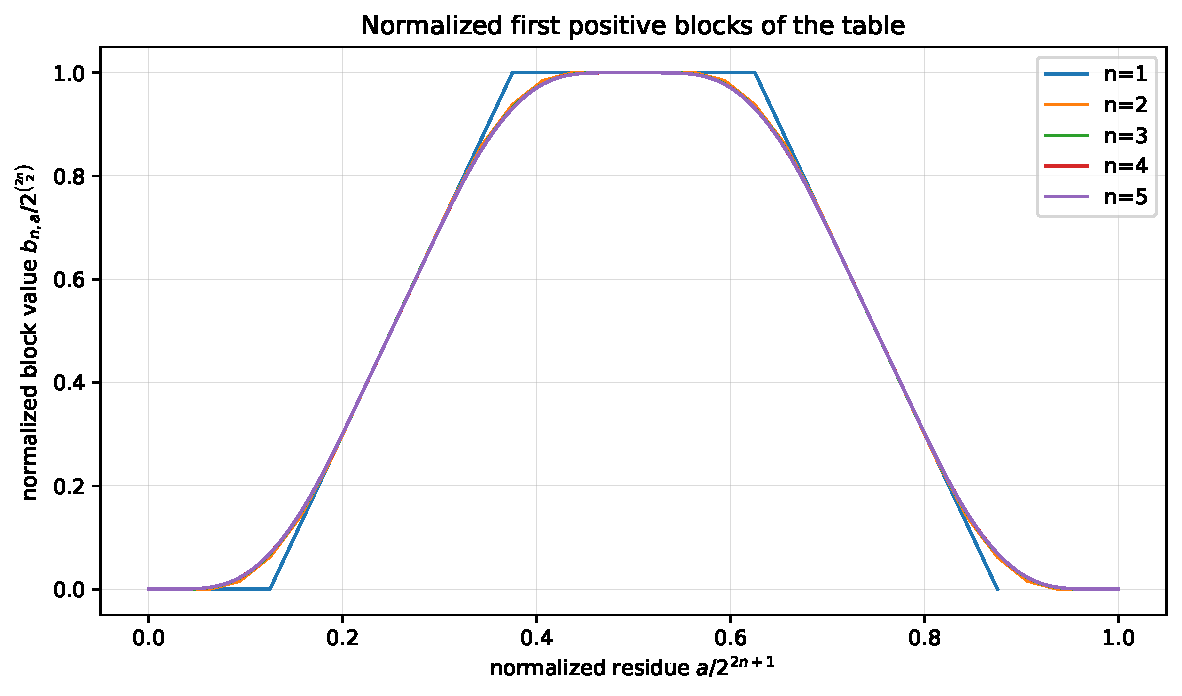
\includegraphics[width=0.94\textwidth]{figures/a_row_profiles.pdf}
\caption{Normalized first positive blocks for \(n=1,\ldots,5\), generated by
\texttt{experiments.py}.  The central plateau has exact width
\((2n+1)/2^{2n+1}\), and the mirror/complement laws hold before taking a
limit.}
\label{a:fig:row-profiles}
\end{figure}
% ---- hand chunk 61-rowdata-lead.tex ----

\section{The first nontrivial blocks and a table of the diagonal array}
In the second report's notation, $H_a(z)=Q_{a+1}(z)$ is the block polynomial
of order $a+1$, $B=2^{2n+1}=L_n$ the block length of row $n$, and the
diagonal-offset coefficients are $\Diag_r(n)=\eps_qq_{2n+1,a}$ for
$r=qL_n+a$.

% ---- B lines 1206--1241 ----
\begin{example}[The first nontrivial finite blocks]
For $n=1$, $B=8$ and
\[
 H_2(z)=(1+z)(1+z+z^2+z^3)
       =1+2z+2z^2+2z^3+z^4.
\]
Thus the diagonal-offset block is
\[
 1,2,2,2,1,0,0,0,
\]
followed by its negative, then by blocks with signs $-1,+1,\ldots$ according
to $\eps_q$.  For $n=2$, $B=32$ and the plateau height is
$2^{\binom42}=64$, attained at diagonal offsets $11,12,13,14,15$.
(The final offsets $27,28,29,30,31$ are instead the zero window.)
\end{example}

A small portion of the diagonal-coordinate table
$(\Diag_m(n))_{n,m\ge0}$ is displayed below.  Rows $n=0$ and $n=1$ already
show the signed block repetition, while larger rows have not yet reached
their first plateau within the displayed window.

\begin{center}
\scriptsize
\setlength{\tabcolsep}{3.6pt}
\begin{tabular}{c|rrrrrrrrrrrrrrrr}
\toprule
$n\backslash m$&0&1&2&3&4&5&6&7&8&9&10&11&12&13&14&15\\
\midrule
0&1&0&-1&0&-1&0&1&0&-1&0&1&0&1&0&-1&0\\
1&1&2&2&2&1&0&0&0&-1&-2&-2&-2&-1&0&0&0\\
2&1&4&9&16&24&32&40&48&55&60&63&64&64&64&64&64\\
3&1&6&20&50&104&190&316&490&719&1008&1360&1776&2256&2800&3408&4080\\
4&1&8&35&112&293&664&1351&2528&4424&7328&11592&17632&25928&37024&51528&70112\\
\bottomrule
\end{tabular}
\end{center}
% ---- B lines 1868--1924 ----
\chapter{Connection with the Fabius and Rvachev approximation layer}
\label{b:sec:fabius}\label{ch:fabius}

The diagonal theory is purely discrete, but it lands exactly on the finite
polynomials used in the repository's Fabius--Rvachev approximants.  The Lean
formalization proves that the order-$k$ iterated prefix coefficients below the
first dyadic cutoff are the coefficients of the approximation polynomial
$p_{k-1}$, and that division by
$2^{\binom{k-1}{2}}$ gives the corresponding step-approximant values at cell
centers \cite{proveit-approx}.

For the odd order $k=2n+1$ considered here, the finite approximation
polynomial is precisely
\begin{equation}
 p_{2n}(z)=H_{2n}(z)
 =\prod_{j=1}^{2n}(1+z+\cdots+z^{2^j-1}).
 \label{b:eq:p-H}
\end{equation}
Therefore, whenever $0\le m<2^{2n+1}$,
\begin{equation}
 \Diag_m(n)=[z^m]p_{2n}(z),
 \label{b:eq:D-approx-coeff}
\end{equation}
and the normalized step height is
\begin{equation}
 \frac{\Diag_m(n)}{2^{\binom{2n}{2}}}.
 \label{b:eq:normalized-edge}
\end{equation}
The normalizing denominator is exactly the plateau height $C$ in
\eqref{a:eq:Mn-definition}.  Thus the complement law
\eqref{a:eq:row-complement} becomes a normalized reflection around $1/2$,
and the central plateau \eqref{a:eq:row-plateau} becomes the level $1$.

For a fixed diagonal offset $m$, combine \eqref{c:eq:diag-asymp} with
$C=2^{n(2n-1)}$ to obtain
\begin{equation}
 \frac{\Diag_m(n)}{2^{\binom{2n}{2}}}
 =\frac{2^mn^m}{m!}\,2^{-n(2n-1)}
 \left(1+\frac{m(m-1)}{4n}+\bigO(n^{-2})\right).
 \label{b:eq:normalized-diagonal-asymptotic}
\end{equation}
Hence every fixed number of coefficient cells from the left edge is
suppressed by a quadratic exponential in $n$, up to a polynomial factor.
This is an exact quantitative boundary-layer statement for the finite
approximants.  It is consistent with the infinite-order flatness of the
limiting Fabius/Rvachev functions, but it should not be confused with an
asymptotic at a fixed spatial argument: the cell represented by a fixed $m$
moves toward the support endpoint as the grid is refined.

The block factorization also clarifies why the early repeated-summation
picture sees the Fabius shape at all.  After division by $H_{2n}(1)$, the coefficients of $H_{2n}$ are the
probability mass function of a sum of independent discrete uniforms on
$\{0,\ldots,2^j-1\}$, while the normalized limit is related to the continuous
sum of geometrically scaled uniforms appearing in the probability model of
Rvachev's up-function.  The present volume does not reprove that analytic
limit; it isolates the exact finite coefficient algebra on which that limit
acts.
% ---- hand chunk 70-fabius-c-lead.tex ----

\section{Exact row--histogram identification and the table limits}
The identification is exact at the level of cell samples, not only in the
limit; in the following, the pulse polynomial of order $r$ is $Q_r$ of
\eqref{a:eq:Qh-definition}, with coefficients $a_{r,b}=q_{r,b}$.

% ---- C lines 1759--1862 ----
The finite pulse occurring in row \(n\) is not merely analogous to the
approximants in the Fabius--Rvachev theory: it is exactly the even-indexed
subsequence of those approximants.  This identifies the correct shift and
normalization of the table without guesswork.

Let \(\Up\) denote Rvachev's even, compactly supported function, normalized
by \(\Up(0)=1\), and let \(F\) denote the bounded Fabius function on
\([0,1]\), so that
\begin{equation}
 F(x)=\Up(x-1)\qquad(0\leq x\leq1).                       \label{c:eq:F-up}
\end{equation}
These are the classical functions introduced from different viewpoints by
Fabius and the Rvachevs; their arithmetic relation with signed Thue--Morse
prefix sums is developed in detail in \cite{fabius,rvachev1971,arias2018,proveit}.

For the table row \(n\), retain
\begin{equation}
 B_n=2^{2n+1},\qquad H_n=2^{2n},\qquad
 M_n=2^{\binom{2n}{2}}.                                   \label{c:eq:BHM-row}
\end{equation}
The polynomial \(\A_{2n+1}\) of \cref{a:eq:Qh-definition} is precisely the finite
step polynomial usually denoted \(\mathcal P_{2n}\).  Its degree is
\begin{equation}
 G_n=B_n-2n-2.                                             \label{c:eq:Gn}
\end{equation}
For \(0\leq m\leq G_n\), put \(k=n+1+m\).  The standard centered cell
coordinate attached to coefficient \(m\) is
\begin{equation}
 \xi_{n,m}=\frac{2m-G_n}{B_n}
           =\frac{2k-B_n}{B_n}.                           \label{c:eq:row-center}
\end{equation}
Thus the shift by \(n+1\) in \cref{a:eq:row-prefix-identification} exactly cancels the
centering correction in the continuous approximation.

\begin{proposition}[Exact row--histogram identification]
\label{c:prop:row-histogram}
At every coefficient center \(\xi_{n,m}\), the normalized centered
histogram approximant \(\mathcal W_{2n}\) satisfies
\begin{equation}
 \mathcal W_{2n}(\xi_{n,m})
 =\frac{a_{2n+1,m}}{M_n}
 =\frac{s_{n,n+1+m}}{M_n}.                                \label{c:eq:row-histogram}
\end{equation}
In particular, the positive part of the first table block, after division
by its exact height \(M_n\), is the level-\(2n\) Rvachev histogram sampled
at its cell centers.
\end{proposition}

\begin{proof}
The coefficient identity
\(a_{2n+1,m}=T_{m}^{(2n+1)}\) in the first dyadic block follows from
\cref{a:eq:general-signed-block}.  The table identity
\(s_{n,n+1+m}=T_{m}^{(2n+1)}\) is \cref{a:eq:row-prefix-identification}.  Finally, the
histogram normalization at level \(N=2n\) is
\[
 \frac{2^{N}}{2^{\binom{N+1}{2}}}
 =\frac1{2^{\binom N2}}=\frac1{M_n},
\]
and its center formula reduces to \cref{c:eq:row-center}.
\end{proof}

The relation can be stated without introducing the intervening histogram.
It gives a direct approximation algorithm using only the table itself.

\begin{theorem}[Table limits to \(\Up\) and \(F\)]
\label{c:thm:table-fabius-limit}
For \(0\leq x\leq1\), define
\begin{align}
 R_n(x)&=\frac{s_{n,\,n+1+\lfloor B_nx\rfloor}}{M_n},      \label{c:eq:Rn}\\
 F_n(x)&=\frac{s_{n,\,n+1+\lfloor H_nx\rfloor}}{M_n}.      \label{c:eq:Fn}
\end{align}
Then, pointwise,
\begin{align}
 R_n(x)&\longrightarrow \Up(2x-1),                        \label{c:eq:Rn-limit}\\
 F_n(x)&\longrightarrow F(x).                             \label{c:eq:Fn-limit}
\end{align}
No assertion of a uniform convergence rate is implicit in these formulas.
\end{theorem}

\begin{proof}
By \cref{a:eq:row-prefix-identification},
\[
 R_n(x)=
 \frac{T_{\lfloor2^{2n+1}x\rfloor}^{(2n+1)}}
      {2^{\binom{2n}{2}}}.
\]
This is exactly the corrected prefix-grid sample from the repository at
level \(2n\).  The proved corrected convergence theorem there gives
\(R_n(x)\to\Up(2x-1)\) on \([0,1]\) \cite{proveit}.  Since
\(F_n(x)=R_n(x/2)\), relation \cref{c:eq:F-up} gives
\[
 F_n(x)\longrightarrow \Up(x-1)=F(x).
\]
\end{proof}

This theorem clarifies the roles of the two limits studied in the volume.
A fixed row and varying column exhibit the compact pulse and its signed
block repetitions.  A fixed diagonal and varying row produce the
polynomials \(\Diag_q(n)\).  The Fabius limit instead lets the shifted
column \(q\) grow exponentially with the row, at the scale
\(q\asymp2^{2n}\).  Thus fixed-diagonal asymptotics such as
\cref{c:eq:diag-asymp} and the continuum limit are complementary scaling
regimes of the same exact array.
% ---- A lines 1420--1545 ----
\chapter{Algorithms and Wolfram Language implementation}\label{ch:algorithms}

\section{Replacing the finite list of diagonal rules}

The eight hand-written diagonal branches can be replaced by one exact
definition.  The following Wolfram Language code uses \texttt{Pochhammer} for
the rising factorial and memoizes each symbolic polynomial.

\begin{lstlisting}[language=Mathematica,caption={Exact polynomial for every diagonal.}]
ClearAll[tmSign, diagonalPolynomial, x];

tmSign[q_Integer?NonNegative] := (-1)^ThueMorse[q];

diagonalPolynomial[0] = 1;
diagonalPolynomial[r_Integer?Positive] :=
  diagonalPolynomial[r] =
    Expand@Sum[
      tmSign[q] Pochhammer[2 x, r - 2 q]/Factorial[r - 2 q],
      {q, 0, Quotient[r, 2]}
    ];

ClearAll[sByDiagonal];
sByDiagonal[n_Integer?NonNegative, k_Integer?NonNegative] /; k <= n := 0;
sByDiagonal[n_Integer?NonNegative, k_Integer?NonNegative] :=
  diagonalPolynomial[k - n - 1] /. x -> n;
\end{lstlisting}

This route is ideal when \(k-n\) is small and \(n\) is large: its work depends
on the diagonal offset, not on the row index.  A direct numeric form avoids
symbolic expansion:

\begin{lstlisting}[language=Mathematica,caption={Direct exact evaluation of one diagonal entry.}]
ClearAll[sDiagonalValue];
sDiagonalValue[n_Integer?NonNegative, k_Integer?NonNegative] /; k <= n := 0;
sDiagonalValue[n_Integer?NonNegative, k_Integer?NonNegative] := Module[
  {r = k - n - 1},
  Sum[
    (-1)^ThueMorse[q] Binomial[2 n + r - 2 q - 1, r - 2 q],
    {q, 0, Quotient[r, 2]}
  ]
];
\end{lstlisting}

\section{Generating consecutive polynomials by the ruler recurrence}

When all diagonals through \(r=R\) are wanted, the recurrence
\eqref{a:eq:ruler-recurrence} reuses previous results and exposes the valuation
structure.

\begin{lstlisting}[language=Mathematica,basicstyle=\ttfamily\footnotesize,caption={Ruler-function recurrence for consecutive diagonals.}]
ClearAll[diagonalRuler, x];
diagonalRuler[0] = 1;
diagonalRuler[r_Integer?Positive] :=
  diagonalRuler[r] = Expand[
    Sum[
      (2 x + 2 - 2^(IntegerExponent[m, 2] + 1))
        diagonalRuler[r - m],
      {m, 1, r}
    ]/r
  ];
\end{lstlisting}

The recurrence is triangular and requires \(R(R+1)/2\) polynomial
multiplications by linear factors.  For one isolated diagonal,
\eqref{a:eq:main-diagonal} is usually shorter; for a full prefix of the family,
the ruler recurrence is usually preferable.

\section{Precomputing a complete row block}

For fixed moderate \(n\) and many arbitrary \(k\), precompute the one positive
block \(B_n\) and use the signed block law.

\begin{lstlisting}[language=Mathematica,caption={Block-based exact table lookup.}]
ClearAll[z, rowBlockPolynomial, rowBlock, sByBlock];

rowBlockPolynomial[n_Integer?NonNegative] :=
  rowBlockPolynomial[n] = Expand[
    z^(n + 1) Product[
      Sum[z^a, {a, 0, 2^j - 1}],
      {j, 1, 2 n}
    ]
  ];

rowBlock[n_Integer?NonNegative] := rowBlock[n] = Module[
  {len = 2^(2 n + 1)},
  PadRight[CoefficientList[rowBlockPolynomial[n], z], len]
];

sByBlock[n_Integer?NonNegative, k_Integer?NonNegative] := Module[
  {len = 2^(2 n + 1), q, a},
  q = Quotient[k, len];
  a = Mod[k, len];
  (-1)^ThueMorse[q] rowBlock[n][[a + 1]]
];
\end{lstlisting}

The polynomial expansion shown here is concise and suitable for presentation.
For larger \(n\), the companion Python code computes the same coefficient list
by repeated convolution with all-one windows, using a sliding sum so each
factor is processed in linear time in the current output length.

\section{Useful additional acceleration rules}

The structural theorem supplies exact branches that are absent from the
original listing.  Inside the first block and for \(n\ge1\),
\begin{align}
 s_{n,L_n/4}&=M_n/2,
 \label{a:eq:wl-quarter-rule}\\
 s_{n,a}&=M_n
 \quad\text{for }L_n/2-n\le a\le L_n/2+n,
 \label{a:eq:wl-plateau-rule}\\
 s_{n,a}&=0
 \quad\text{for }0\le a\le n
 \text{ or }L_n-n\le a<L_n.
 \label{a:eq:wl-zero-rule}
\end{align}
Together with the stronger full-half complement
\eqref{a:eq:row-complement}, these can reduce recursion depth substantially.
Care is required to order conditional definitions so that fixed points such as
\(a=L_n/4\) are handled before a symmetry branch referring to themselves.

The standalone file \texttt{thue\_morse\_table.wl} packages these identities in
\texttt{sFast[n,k]}.  It first reduces \(k\) to its signed dyadic block, maps the
local residue through the zero, plateau, reflection, and complement laws into the
first quarter, and finally calls the finite diagonal formula.  Thus an arbitrary
entry can be evaluated without constructing the complete exponentially long block.
% ---- hand chunk 80-algorithms-b-lead.tex ----

\section{Block reduction in the diagonal coordinate}
The direct sum \eqref{a:eq:main-diagonal} has only $\lfloor r/2\rfloor+1$
summands, but it is unsuitable when the reduced offset is very large. The
block law of \cref{ch:rows} first reduces an arbitrary offset modulo the
block length, and a second idea removes the remaining dependence on the
offset altogether.

% ---- B lines 1722--1729 ----
The block law \eqref{a:eq:row-signed-block} first reduces an arbitrary $m$ modulo
$B=2^{2n+1}$:
\begin{equation}
 \Diag_m(n)=\eps_{\lfloor m/B\rfloor}\Diag_{m\bmod B}(n).
 \label{b:eq:diagonal-block-reduction}
\end{equation}
Unlike the original code's block rule, this version acts directly on the
natural diagonal offset.  It avoids bookkeeping caused by the shift $n+1$.
% ---- B lines 1731--1866 ----
\section{Logarithmic-time signed prefix moments}

The direct sum is still unsuitable when the reduced offset is very large.
The key observation is that, for fixed $n\ge1$, its binomial kernel is a
polynomial of degree $2n-1$ in the Thue--Morse index $q$:
\begin{equation}
 \binom{2n+m-2q-1}{m-2q}
 =\binom{2n+m-2q-1}{2n-1}
 =\sum_{d=0}^{2n-1}c_d(m,n)q^d.
 \label{b:eq:kernel-polynomial}
\end{equation}
Thus only finitely many signed prefix moments are required.

\begin{definition}[Signed Thue--Morse prefix moments]
For $N,d\in\N$, let
\begin{equation}
 M_d(N)=\sum_{q=0}^{N-1}\eps_qq^d.
 \label{b:eq:prefix-moment}
\end{equation}
The sum is exclusive at $N$; $M_d(0)=0$.
\end{definition}

\begin{theorem}[Binary divide-and-conquer recurrence]
\label{b:thm:moment-recurrence}
For $N,d\in\N$,
\begin{align}
 M_d(2N)
 &=-\sum_{j=0}^{d-1}\binom dj2^jM_j(N),
 \label{b:eq:moment-even}\\
 M_d(2N+1)
 &=M_d(2N)+\eps_N(2N)^d.
 \label{b:eq:moment-odd}
\end{align}
The sum in \eqref{b:eq:moment-even} is empty when $d=0$.
\end{theorem}

\begin{proof}
Pair the terms with indices $2q$ and $2q+1$ and use
\eqref{a:eq:tm-recursion}:
\begin{align*}
 M_d(2N)
 &=\sum_{q=0}^{N-1}
   \left(\eps_{2q}(2q)^d+\eps_{2q+1}(2q+1)^d\right)\\
 &=\sum_{q=0}^{N-1}\eps_q\left((2q)^d-(2q+1)^d\right)\\
 &=-\sum_{j=0}^{d-1}\binom dj2^j
     \sum_{q=0}^{N-1}\eps_qq^j.
\end{align*}
The highest-degree terms cancel.  Adding the final term at index $2N$ gives
\eqref{b:eq:moment-odd}.
\end{proof}

Let $L=\lfloor m/2\rfloor+1$.  Combining
\eqref{b:eq:kernel-polynomial} with \eqref{b:eq:prefix-moment} gives
\begin{equation}
 \boxed{\quad
 \Diag_m(n)=\sum_{d=0}^{2n-1}c_d(m,n)M_d(L)
 \qquad(n\ge1).
 \quad}
 \label{b:eq:moment-evaluator}
\end{equation}
The recursion depth for $M_d(L)$ is $O(\log L)$.  At each level, computing
all moments through degree $2n-1$ by \eqref{b:eq:moment-even} uses
$O(n^2)$ arithmetic operations.  Ignoring integer multiplication bit costs,
the evaluator therefore uses
\begin{equation}
 O(n^2\log m)
 \label{b:eq:moment-complexity}
\end{equation}
exact arithmetic operations, rather than $O(m)$ summands.

\begin{algorithm}[Hybrid evaluator]
\label{b:alg:hybrid}
Given $n,k\in\N$:
\begin{enumerate}
 \item If $k\le n$, return $0$.
 \item Set $m=k-n-1$, $B=2^{2n+1}$, and write $m=qB+r$.
 \item Compute the core value $\Diag_r(n)$ by the direct sum if $r$ is below
       a chosen small cutoff; otherwise use \eqref{b:eq:moment-evaluator}.
 \item Return $\eps_q\Diag_r(n)$.
\end{enumerate}
\end{algorithm}

The cutoff only chooses between two exact algorithms; it does not affect the
result.  The supplied implementation uses $128$ by default.

\begin{lstlisting}[style=code,language=Wolfram]
tmPrefixMoments[0, maxDegree_Integer?NonNegative] :=
  ConstantArray[0, maxDegree + 1];

tmPrefixMoments[length_Integer?Positive, maxDegree_Integer?NonNegative] :=
  tmPrefixMoments[length, maxDegree] = Module[
    {half = Quotient[length, 2], lower, paired},
    lower = tmPrefixMoments[half, maxDegree];
    paired = Table[
      If[d == 0, 0,
        -Sum[Binomial[d, j] 2^j lower[[j + 1]], {j, 0, d - 1}]
      ],
      {d, 0, maxDegree}
    ];
    If[OddQ[length],
      paired += tmSign[half] Table[(2 half)^d, {d, 0, maxDegree}]
    ];
    paired
  ];
\end{lstlisting}

For $n\ge1$, the polynomial coefficients $c_d(m,n)$ are obtained exactly
from
\[
 \frac{1}{(2n-1)!}\prod_{j=1}^{2n-1}(m-2q+j).
\]
The full source file \texttt{diagonal\_polynomials.wl} contains this
contraction, block reduction, a compact replacement for the original
\texttt{s}, and a literal repeated-prefix reference implementation.

\section{Memory and implementation notes}

The memoized moment routine stores vectors keyed by the pair
$(N,d_{\max})$.  A single query touches only the binary ancestors
$N,\lfloor N/2\rfloor,\lfloor N/4\rfloor,\ldots$, so its live recursion
depth is logarithmic.  For a long batch with many unrelated degree bounds,
one may remove memoization or cache moments at a fixed maximum degree and
truncate as needed.

Exact integer sizes can be very large.  Complexity
\eqref{b:eq:moment-complexity} counts arithmetic operations, not bit
operations; this is the appropriate distinction because the output itself
may contain thousands or millions of bits.  The algorithm avoids artificial
work proportional to the index $m$, but it cannot avoid the cost of storing
the exact answer.

The local recurrence \eqref{b:eq:local-pde} remains preferable when a dense
rectangular region is desired.  The moment method is designed for sparse
random access to isolated entries.  The diagonal polynomial and Newton--Bell
methods are designed for symbolic dependence on $n$.  Keeping these use cases
separate leads to simpler and faster code.
% ---- hand chunk 81-algorithms-c-lead.tex ----

The exact theorems of \cref{ch:arithmetic,ch:roots} also translate directly
into inexpensive integer tests; the following routines, from the third
report's implementation, are retained as
\path{verification/source3/thue_morse_diagonals.wl}.

% ---- C lines 1582--1649 ----
\section{Root and denominator utilities}

The exact theorems translate directly into inexpensive integer tests.

\begin{lstlisting}[language=Wolfram,caption={Exact rational-root tests and coefficient denominator.}]
ClearAll[halfGridRootIndices, halfGridFactor,
  negativeHalfGridValue, negativeHalfGridRootQ,
  minimalMonomialDenominator];

halfGridRootIndices[d_Integer?Positive] := Module[
  {q = d - 1},
  If[q == 0, {},
    Select[Range[0, q - 1],
      Mod[q, 2^(# + 1)] >= 2^(# + 1) - (# + 1) &]
  ]
];

halfGridFactor[d_Integer?Positive, var_: x] :=
  Times @@ (2 var - # & /@ halfGridRootIndices[d]);

(* The point tested here is x=-m/2, m>=1. *)
negativeHalfGridValue[d_Integer?Positive,
    m_Integer?Positive] := Module[{q = d - 1},
  Sum[(-1)^j Binomial[m - 1, j]
    If[q - j < 0, 0, tmSign[q - j]], {j, 0, m - 1}]
];

negativeHalfGridRootQ[d_Integer?Positive,
    m_Integer?Positive] :=
  PossibleZeroQ[negativeHalfGridValue[d, m]];

minimalMonomialDenominator[d_Integer?Positive] := Module[
  {q = d - 1, c, v2},
  c = Ceiling[q/2];
  v2 = IntegerExponent[Factorial[q], 2];
  Factorial[q]/2^Min[v2, c]
];
\end{lstlisting}

For instance,
\begin{lstlisting}[language=Wolfram]
Table[
  {d, halfGridRootIndices[d],
      Factor[halfGridFactor[d, x]],
      minimalMonomialDenominator[d]},
  {d, 1, 32}
]
\end{lstlisting}
returns the exact nonnegative rational factor and least coefficient
denominator for each of the first thirty-two diagonals without factoring the
full polynomial.  Negative candidates are tested with
\texttt{negativeHalfGridRootQ[d,m]}, which evaluates the polynomial at
\(-m/2\) by the finite-difference formula rather than by expansion.

\section{Independent consistency checks}

The supplied \texttt{thue\_morse\_diagonals.wl} file also contains a literal
memoized prefix-sum implementation and the following checks:
\begin{lstlisting}[language=Wolfram]
verifyPromptDiagonals[]
verifyClosedFormula[5, 50]
verifyRecurrence[5, 50]
\end{lstlisting}
The first compares the general formula with all eight explicit polynomials of
the originating program.  The second compares the sparse formula, literal repeated prefix
sums, and the signed block formula.  The third verifies the weighted row
recurrence \cref{a:eq:weighted-recurrence}.  These are regression tests; the preceding
sections provide the proofs.
% ---- A lines 1547--1588 ----
\chapter{Computational verification}\label{ch:verification}

The archive accompanying this volume contains
\texttt{experiments.py}.  Its identities are checked with Python integers and
SymPy exact rationals; floating-point arithmetic is used only to draw
Figure~\ref{a:fig:row-profiles}.  The program performs the following independent
comparisons.

\begin{enumerate}
\item It builds the table from the original weighted recurrence using prefix
sums to evaluate each weighted convolution in constant time after preprocessing
one row.

\item It evaluates \(\Diag_{k-n-1}(n)\) directly from
\eqref{a:eq:main-diagonal} and compares every tested entry with the recurrence.

\item It constructs the finite block \(B_n\) by sliding-window convolutions
and compares the signed-block lookup with both previous methods.

\item It mirrors the branch order of the Wolfram Language hybrid evaluator
\texttt{sFast}, checks every residue of the tested row blocks, and then checks
several complete signed repetitions.

\item It constructs the same diagonal polynomials independently from the
ruler recurrence and verifies the half-step and differential identities
symbolically.

\item It checks support, reflection, complement, plateau, total mass,
multiplicities, and distinct-value counts for several rows and for arbitrary
summation orders \(h\) through the tested range.

\item It verifies the nonnegative half-integer root criterion and the negative
half-integer finite-difference formula, including the two valuation criteria
\eqref{a:eq:x-minus-one-root}--\eqref{a:eq:x-minus-two-root}.
\end{enumerate}

A successful run prints
\begin{lstlisting}
All exact checks passed.
\end{lstlisting}
and writes a text report of the initial factorizations.  These experiments are
regression checks rather than substitutes for the proofs above.
% ---- hand chunk 90-verification-programs.tex ----

\section{The three retained verification programs}
Each source shipped an exact verification program together with a Wolfram
Language implementation, and all three are retained unchanged under
\path{verification/} in the package directory, with the outputs of the runs
that accompanied the sources. Their checks overlap, and they were written
independently, so agreement between them is evidence about the
normalizations rather than about a shared implementation.
\begin{itemize}
\item \path{verification/source1/experiments.py} is the program described
above, with \path{thue_morse_table.wl} (the hybrid evaluator
\texttt{sFast}) and \path{verification_report.txt}.
\item \path{verification/source2/diagonal_polynomials.py} verifies, in
exact SymPy arithmetic, the direct and Newton--Bell generators, the
half-step law, literal repeated prefix summation, finite-block reduction,
the prefix-moment evaluator of \cref{ch:algorithms}, primitive normalization,
exact denominators, and both half-grid formulas; run with
\texttt{--max-degree 12 --verify}, and with \texttt{--scan-negative-half}
for the finite scan reported after \cref{b:conj:no-negative-strict-half}
(no counterexample for odd $b\le63$, $m\le10000$). Its Wolfram Language
companion \path{diagonal_polynomials.wl} contains the moment contraction,
block reduction, a compact replacement for the original \texttt{s}, and a
literal repeated-prefix reference implementation; \path{VERIFICATION.txt}
records the commands, versions and results.
\item \path{verification/source3/diagonal_analysis.py} performs the checks
listed next, writes \path{generated/verification_report.txt},
\path{generated/diagonal_polynomials.csv} and
\path{generated/half_grid_roots.csv}, and regenerates the normalized-pulse
figure; \path{thue_morse_diagonals.wl} holds the routines of
\cref{ch:algorithms} and the consistency checks
\texttt{verifyPromptDiagonals}, \texttt{verifyClosedFormula} and
\texttt{verifyRecurrence}.
\end{itemize}

% ---- C lines 1653--1734 ----
\section{Exact Python verification}

The archive includes \texttt{diagonal\_analysis.py}.  It uses Python integers
for the discrete checks and SymPy rational polynomials for symbolic
expansion.  Running
\begin{lstlisting}[language=Python]
python diagonal_analysis.py --output-dir generated --max-table-q 20
\end{lstlisting}
creates:
\begin{itemize}[leftmargin=2em]
\item \texttt{verification\_report.txt},
\item \texttt{diagonal\_polynomials.csv},
\item \texttt{half\_grid\_roots.csv}, and
\item the PDF and PNG versions of the normalized-pulse figure, retained as \path{figures/c_normalized_row_pulses.pdf}.
\end{itemize}

The bundled run performed the following exact checks.

\begin{enumerate}[leftmargin=2.2em]
\item The sparse formula, literal repeated prefix sums, and signed block
formula agree for \(0\leq n\leq5\), \(0\leq k\leq70\).
\item The weighted recurrence agrees on the same range for
\(1\leq n\leq5\).
\item Polynomial evaluation agrees with the integer sparse sum for
\(0\leq q\leq30\).
\item The nonnegative half-grid zero criterion agrees for
\(0\leq q,m\leq30\).
\item The negative half-grid finite-difference formula agrees with exact
polynomial evaluation for \(0\leq q\leq30\), \(1\leq m\leq16\).
\item The trailing-ones negative-root theorem agrees for exponents
\(2\leq a\leq9\) in four consecutive dyadic blocks.
\item The exact minimal denominator formula agrees with coefficient
inspection for \(0\leq q\leq24\).
\item Pulse support, positivity, palindromy, mass, maximum, and plateau length
agree for prefix orders \(1\) through \(10\).
\end{enumerate}

All assertions use exact equality.  The numerical root quoted after
\cref{a:thm:half-root} is the only floating-point datum in the main
mathematical discussion.

\section{Selected continued factorizations}

The polynomial law continues well beyond the eight hand-entered cases.  The
following table records exact rational linear factors found by symbolic
factorization.  The nonnegative factors are predicted a priori by
\cref{a:thm:half-root}; negative factors illustrate the additional
structure still to be classified.

\begin{longtable}{c c p{0.52\textwidth} c}
\caption{Selected exact rational factors of \(\Diag_q\).\label{c:tab:factorizations}}\\
\toprule
\(d\)&\(q\)&rational linear factor product&residual degree\\
\midrule
\endfirsthead
\toprule
\(d\)&\(q\)&rational linear factor product&residual degree\\
\midrule
\endhead
1&0&\(1\)&0\\
2&1&\(x\)&0\\
3&2&\((x+1)(2x-1)\)&0\\
4&3&\(x(x+2)(2x-1)\)&0\\
5&4&\(1\)&4\\
6&5&\(x(x-1)\)&3\\
7&6&\((x-1)(x+1)(2x-1)\)&3\\
8&7&\(x(x-1)(x+2)(2x-1)\)&3\\
9&8&\(x+1\)&7\\
10&9&\(x(x+2)\)&7\\
11&10&\((x+1)(x+3)(2x-1)\)&7\\
12&11&\(x(x+2)(x+4)(2x-1)\)&7\\
13&12&\((x+5)(2x-3)\)&10\\
14&13&\(x(x-1)(x+6)(2x-3)\)&9\\
15&14&\((x-1)(x+1)(x+7)(2x-3)(2x-1)\)&9\\
16&15&\(x(x-1)(x+2)(x+8)(2x-3)(2x-1)\)&9\\
\bottomrule
\end{longtable}

The factors in \cref{c:tab:factorizations} were verified by exact polynomial
division.  No irreducibility claim is made for the residual factors unless a
computer algebra system has certified it over \(\Q\); the table is intended
to display recurring linear structure, not to replace the general theorems.
% ---- A lines 1590--1625 ----
\chapter{Further deductions and research directions}\label{ch:future}

\section{Polynomial interpolation in a discrete parameter}

The variable \(x\) is not merely a formal row coordinate.  Under
\(h=2x+1\), it continuously interpolates the discrete order of summation.  The
half-step recurrence is exactly the identity that one additional summation in
\(h\) produces one lower-index coefficient after taking a difference in the
order parameter.  This may be useful when comparing different repeated-
integration normalizations in the Fabius corpus.

\section{Root automata and residual factors}

The nonnegative half-integer roots are completely classified by a terminal
block condition.  At a fixed negative half-integer, the zero test is a finite
linear combination of a bounded window of Thue--Morse signs.  This suggests a
systematic finite-automaton study of the residual linear factors of
\(\Diag_r\) as \(r\) varies.  The examples \(x+1\) and \(x+2\) already reduce
to elementary \(2\)-adic valuation parity.  Higher backward differences
produce richer but still finite digital conditions.

\section{Other Mahler products}

The deflation theorem \eqref{a:eq:general-deflation} applies whenever a base
generating function contains a factor \((1-z)^c\) and then contracts to
\(z^b\).  For products of the form
\[
 E_b(z)=\prod_{j\ge0}(1-z^{b^j}),
 \qquad
 E_b(z)=(1-z)E_b(z^b),
\]
one obtains an analogous sparse diagonal polynomial with degree gaps in
multiples of \(b\).  Finite-level factorization then produces blocks of length
\(b^h\).  Positivity and the exact plateau geometry require additional care
when the quotient factors are no longer all-one intervals, but the polynomial
mechanism survives unchanged.
% ---- B lines 1933--1984 ----
\section{Scaling regimes beyond fixed diagonals}

The fixed-$m$ asymptotic \eqref{c:eq:diag-asymp} is only the extreme left edge.
There are at least four natural regimes for $m=m(n)$:
\begin{enumerate}
 \item $m$ fixed;
 \item $m\to\infty$ but $m=o(2^n)$, where only the first few geometric upper
       bounds in \eqref{a:eq:bounded-composition} are active;
 \item $m$ proportional to the standard deviation of the restricted-uniform
       sum, where a local central limit theorem should control $h_{2n,m}$;
 \item $m$ within $O(n)$ of the exact plateau and zero-run boundaries, where
       finite edge corrections dominate.
\end{enumerate}
A uniform saddle-point analysis of
$H_{2n}(z)$ could connect the polynomial edge law to the Gaussian bulk and
the exact flat plateau without passing through separate approximations.

\section{Residual factors and zero geometry}

After removing the completely classified nonnegative rational factor
$R_m^+$ and the negative integer factors detected by
\eqref{b:eq:negative-half-value}, the remaining factor often appears
irreducible over $\Q$ in low degrees.  Questions include:
\begin{itemize}
 \item Are all nonnegative half-integer zeros simple?
 \item Can the negative integer roots be characterized by binary automata in
       the pair $(m,r)$ from the binomial sums at $x=-r$?
 \item Does \cref{b:conj:no-negative-strict-half} hold?
 \item What is the limiting distribution of the nonrational complex zeros of
       $\Diag_m$ after an $m$-dependent scaling?
\end{itemize}
The half-step lowering law suggests that finite-difference analogues of
classical results on Appell and Sheffer zero interlacing may be relevant, but
$\TM(z^2)$ is not a positivity-preserving prefactor, so standard real-rooted
arguments do not apply directly.

\section{Automatic and \texorpdfstring{$p$-adic}{p-adic} structure}

The cumulants \eqref{a:eq:ruler-logarithm} depend on $r$ only through $\vtwo(r)$.  This
makes the Newton recurrence an unusual hybrid of Bell-polynomial and
automatic-sequence structure.  It is natural to ask for:
\begin{itemize}
 \item finite automata or linear representations for coefficient residues of
       the primitive polynomials $\Dprim_m$ modulo odd primes;
 \item exact Newton polygons of $\Dprim_m$ at $2$ beyond the coarse bound
       \eqref{b:eq:coefficient-v2-bound};
 \item analogues for generalized base-$b$ Thue--Morse products
       $\prod_{j\ge0}(1-z^{b^j})$ or for weighted digit characters.
\end{itemize}
For a general digit character, the logarithmic cumulants are controlled by
$b$-adic divisibility, so much of the Riordan and Bell machinery survives
with $\vtwo$ replaced by $\nu_b$ and with a different finite block.
% ---- C lines 1870--1948 ----
\section{Binary classification of negative rational factors}

The nonnegative rational factors have the residue-window description
\cref{a:eq:half-root-criterion}.  On the negative side,
\cref{a:eq:negative-half-formula} gives a complete finite-difference test, but it
is not yet a comparably transparent description in the binary digits of
\(q\) and \(m\).  A natural next problem is to characterize the zero set
\begin{equation}
 \left\{(q,m)\in\N\times\N_{>0}:
   \nabla^{m-1}\eps_q=0\right\}                           \label{c:eq:negative-zero-set}
\end{equation}
in terms of carries, complemented suffixes, or a finite collection of
binary recursions.  The trailing-ones theorem
\cref{c:thm:negative-family} is one infinite stratum of this set.

Because \(\eps_q\) is a two-automatic sequence, the bivariate zero mask in
\cref{c:eq:negative-zero-set} is a promising candidate for analysis by
regular-sequence and linear-representation methods.  Even a classification
for fixed \(m\), or for \(m\) restricted to powers of two, would sharpen
the factor tables substantially.

\section{The residual root geometry}

Remove from \(\Diag_q\) every rational linear factor detected by
\cref{a:thm:half-root,a:thm:negative-half}.  The remaining factor can
have irrational real roots as well as complex-conjugate pairs.  The
following questions are concrete and computationally accessible.

\begin{enumerate}[leftmargin=2.2em]
\item How many real roots can the residual factor have, and how does this
number depend on the binary expansion of \(q\)?
\item Is there a useful vertical strip or parabolic region containing all
roots after centering by the exact mean \(-(q-1)/4\)?
\item Do the empirical root measures have a limiting distribution after an
appropriate scaling in \(q\)?
\item Which diagonals have repeated roots?  The generating and difference
identities provide exact resultant recurrences with which to test
square-freeness.
\end{enumerate}

The exact root moments in \cref{c:eq:root-sum,c:eq:root-square-sum} give two
nontrivial constraints on any proposed limiting law.

\section{Joint asymptotics beyond a fixed diagonal}

Formula \cref{c:eq:diag-asymp} treats \(q\) as fixed while \(n\to\infty\).
The Fabius scaling in \cref{c:thm:table-fabius-limit} instead has
\(q\asymp2^{2n}\).  Between them lie several unexplored regimes:
\begin{equation}
 q=o(n),\qquad q\asymp n,\qquad q\asymp n^2,
 \,\ldots\,,\qquad q\asymp2^{2n}.                         \label{c:eq:scaling-regimes}
\end{equation}
The coefficient integral
\begin{equation}
 \Diag_q(n)=\frac{1}{2\pi i}\oint
  \frac{\K(z^2)}{(1-z)^{2n}}\frac{dz}{z^{q+1}}           \label{c:eq:diag-Cauchy}
\end{equation}
provides a common starting point.  For subexponential \(q\), the saddle
comes mainly from the negative-binomial factor; as it approaches dyadic
scales, zeros and oscillations of the lacunary factor \(\K(z^2)\) can no
longer be treated as a perturbation.  A uniform bridge between these
regimes would connect the polynomial theory directly to the sharp Fabius
asymptotics.

\section{Fast coefficient queries inside one pulse}

Constructing all coefficients of \(\A_r\) costs \(O(2^r)\) memory, although
the sliding-window recurrence is optimal when the whole pulse is required.
For one coefficient \(a_{r,b}\), it should be possible to exploit the
binary expansion of \(b\), palindromy, plateau structure, and recursive
interval convolution to obtain substantially smaller memory use.  Useful
targets include:
\begin{itemize}[leftmargin=2em]
\item a divide-and-conquer exact evaluator for one coefficient;
\item certified modular evaluation followed by Chinese remaindering;
\item asymptotically sharp local-limit estimates with rigorous error terms;
\item an adaptive method that switches between the sparse diagonal sum and
the dyadic pulse representation according to \(q=k-n-1\).
\end{itemize}
% ---- hand chunk 91-directions-formalization.tex ----

\section{Formalization targets}
The repository already crosswalks Lean proofs of the exact prefix formula,
iterated-prefix convolution, finite dyadic quotient, terminal zero run,
signed reversal, finite approximation polynomials, corrected normalization
and step approximants \cite{atlas,proveit-prefix,proveit-approx}. The
statements of this volume reduce to finite sums, polynomial identities,
formal power-series coefficient extraction, and elementary integer
divisibility once those inputs are imported. The natural additions, in
dependency order, are:
\begin{enumerate}
\item the shifted-table identity \eqref{a:eq:row-prefix-identification} and
the local discrete equation \eqref{b:eq:local-pde};
\item a polynomial-valued definition of $\Diag_r$, the generating function
\eqref{a:eq:Sheffer-egf}, the sparse formula \eqref{a:eq:main-diagonal}, and
the evaluation theorem $s_{n,n+1+r}=\Diag_r(n)$;
\item the half-step, ruler and differential recurrences and the diagonal
Mahler equation \eqref{c:eq:diag-mahler};
\item the finite-block theorem \eqref{a:eq:block-factorization} with the
plateau, complement, multiplicity and distinct-value statements for $Q_h$
and $B_n$;
\item the half-grid transposition \eqref{c:eq:transposition}, the exact
half-integer zero criterion, and the negative half-lattice formula;
\item primitive normalization, the exact denominator theorem, and the
rational-root restriction;
\item the trailing-ones negative-root family \eqref{c:eq:negative-family};
\item the signed-prefix-moment recurrences and the correctness of the fast
evaluator;
\item the exact row--histogram identification \eqref{c:eq:row-histogram}
against the existing approximation modules.
\end{enumerate}
None of these is claimed to have been formalized; the list is a technical
implementation guide.

% ---- hand chunk 95-appendix-head.tex ----

\appendix

% ---- A lines 1669--1695 ----
\chapter{A compact theorem dictionary}\label{app:dictionary}

For reference, the principal objects and translations are collected here.

\begin{center}
\begin{tabularx}{\textwidth}{@{}p{0.25\textwidth}X@{}}
\toprule
Object & Exact formula or relation \\
\midrule
Signed Thue--Morse & \(\eps_q=(-1)^{\wt(q)}\) \\
Lacunary series & \(E(z)=\sum_q\eps_qz^q=\prod_{j\ge0}(1-z^{2^j})\) \\
Mahler equation & \(E(z)=(1-z)E(z^2)\) \\
Exclusive prefix & \(S(2q)=0,\ S(2q+1)=\eps_q\) \\
Iterated prefix & \(\sum_r\Prefix_r^{(h)}z^r=E(z)/(1-z)^h\) \\
Row generating function & \(A_n(z)=z^{n+1}E(z)/(1-z)^{2n+1}\) \\
Row/prefix map & \(s_{n,n+1+r}=\Prefix_r^{(2n+1)}\) \\
Diagonal polynomial & \(\Diag_r(x)=[z^r]E(z^2)/(1-z)^{2x}\) \\
Original diagonal \(d\) & \(P_d(x)=\Diag_{d-1}(x)\) \\
Half-step & \(\Diag_r(x)-\Diag_r(x-1/2)=\Diag_{r-1}(x)\) \\
Ruler coefficient & \(\lambda_m(x)=2x+2-2^{\nuTwo(m)+1}\) \\
Ruler recurrence & \(r\Diag_r=\sum_{m=1}^rc_m\Diag_{r-m}\) \\
Row block length & \(L_n=2^{2n+1}\) \\
Row maximum & \(M_n=2^{\binom{2n}{2}}\) \\
Signed block law & \(s_{n,qL_n+a}=\eps_qb_{n,a}\) \\
\bottomrule
\end{tabularx}
\end{center}
% ---- B lines 2050--2091 ----
\chapter{Nonnegative rational factors through \texorpdfstring{$m=31$}{m=31}}
\label{b:app:factor-table}

The following table lists, for each $m$, the set $\mathcal A_m$ of those $a\ge0$ with $m\bmod 2^{a+1}\ge2^{a+1}-a-1$, so that $\prod_{a\in\mathcal A_m}(2x-a)$ is the systematic factor $\Phi_m$ of \eqref{a:eq:Phi-factor}.  The displayed
squarefree product $\prod_{a\in\mathcal A_m}(2x-a)$ contains one copy of every
nonnegative rational linear factor; an empty set means that $\Diag_m$ has no
nonnegative rational zero.

\begin{center}
\small
\begin{longtable}{r@{\quad}l|r@{\quad}l}
\toprule
$m$ & $\mathcal A_m$ & $m$ & $\mathcal A_m$\\
\midrule
\endfirsthead
\toprule
$m$ & $\mathcal A_m$ & $m$ & $\mathcal A_m$\\
\midrule
\endhead
0&$\varnothing$&16&$\varnothing$\\
1&$\{0\}$&17&$\{0\}$\\
2&$\{1\}$&18&$\{1\}$\\
3&$\{0,1\}$&19&$\{0,1\}$\\
4&$\varnothing$&20&$\varnothing$\\
5&$\{0,2\}$&21&$\{0,2\}$\\
6&$\{1,2\}$&22&$\{1,2\}$\\
7&$\{0,1,2\}$&23&$\{0,1,2\}$\\
8&$\varnothing$&24&$\varnothing$\\
9&$\{0\}$&25&$\{0\}$\\
10&$\{1\}$&26&$\{1\}$\\
11&$\{0,1\}$&27&$\{0,1,4\}$\\
12&$\{3\}$&28&$\{3,4\}$\\
13&$\{0,2,3\}$&29&$\{0,2,3,4\}$\\
14&$\{1,2,3\}$&30&$\{1,2,3,4\}$\\
15&$\{0,1,2,3\}$&31&$\{0,1,2,3,4\}$\\
\bottomrule
\end{longtable}
\end{center}

The table makes the nested terminal windows before powers of two visible.  At
$m=2^{a+1}-a-1,\ldots,2^{a+1}-1$, the new root $x=a/2$ appears; lower-period
root patterns continue independently underneath it.
% ---- C lines 2006--2054 ----
\chapter{Formula sheet for implementation}
\label{c:app:formula-sheet}

For convenient reference, the principal formulas are collected here.

\begin{longtable}{p{0.29\textwidth}p{0.65\textwidth}}
\toprule
quantity & exact formula \\
\midrule
\endfirsthead
\toprule
quantity & exact formula \\
\midrule
\endhead
signed Thue--Morse value
& \(\eps_j=(-1)^{\wt(j)}\) \\
order-\(r\) prefix series
& \(\sum_{q\geq0}T_{q}^{(r)}z^q=\K(z)/(1-z)^r\) \\
whole table
& \(s_{n,k}=T_{k-n-1}^{(2n+1)}\) \\
row series
& \(A_n(z)=z^{n+1}\K(z)/(1-z)^{2n+1}\) \\
full bivariate series
& \(\sum s_{n,k}u^nz^k=z(1-z)\K(z)/((1-z)^2-uz)\) \\
positive pulse
& \(\A_r(z)=\prod_{j=1}^{r-1}(1+z+\cdots+z^{2^j-1})\) \\
block law
& \(T_{a2^r+b}^{(r)}=\eps_a[z^b]\A_r(z)\) \\
terminal zero test
& \(T_{a2^r+b}^{(r)}=0\iff b\geq2^r-r\) \\
diagonal polynomial
& \(\Diag_q(x)=\sum_{j\leq q/2}\eps_j\rising{(2x)}{q-2j}/(q-2j)!\) \\
diagonal generating function
& \(\sum_{q\geq0}\Diag_q(x)z^q=\K(z^2)/(1-z)^{2x}\) \\
direct table evaluator
& \(s_{n,k}=\sum_{j\leq(k-n-1)/2}\eps_j
\binom{n+k-2j-2}{k-n-1-2j}\) for \(k>n\) \\
minimal coefficient denominator
& \(q!/2^{\min(\vTwo(q!),\lceil q/2\rceil)}\) \\
nonnegative rational root
& \(m/2\) is a root iff
\(q\bmod2^{m+1}\geq2^{m+1}-(m+1)\) \\
negative rational root
& \(-m/2\) is a root iff
\(\sum_{j=0}^{m-1}(-1)^j\binom{m-1}{j}\eps_{q-j}=0\) \\
Fabius sample
& \(s_{n,n+1+\lfloor2^{2n}x\rfloor}/2^{\binom{2n}{2}}\to F(x)\) \\
\bottomrule
\end{longtable}
% ---- hand chunk 96-provenance.tex ----

\chapter{Source provenance, notation dictionary, and reproducibility}
\label{app:provenance}
\section{Sources and consolidation}
This volume consolidates the three diagonal-polynomial reports filed in
the repository's frontier intake of September 3, 2026, under
\path{drafts/thue-morse/}: \path{thue_morse_diagonal_polynomials}
(\emph{Diagonal Polynomials and Dyadic Block Geometry in Repeated
Thue--Morse Summation}, the spine of this volume),
\path{thue_morse_diagonal_polynomials-2} (\emph{Diagonal Polynomial Laws in
Odd Iterated Thue--Morse Summation: Riordan-array structure, $2$-adic Bell
recurrences, exact arithmetic, and fast Wolfram Language evaluation}), and
\path{thue_morse_diagonal_polynomials_article_and_code} (\emph{Diagonal
Polynomials and Dyadic Block Geometry in Repeated Thue--Morse Prefix
Summation: Exact formulas, denominator laws, rational roots, and fast
Wolfram Language evaluation}). Their \LaTeX{} sources, PDFs and READMEs were
removed when this volume was filed; the repository history retains them.
The verification programs, Wolfram Language files, generated data, and
figures were retained unchanged.

The first report supplies the chapter structure and the statements and
proofs of every result all three shared. The second report contributed the
local discrete equation, the Riordan-array chapter with its general
subdiagonal theorem, the binomial-basis integer coefficients, the partition
and determinant forms of the Bell representation, the half-grid
translation formulas and the integer-step relation, the arithmetic chapter
(primitive normalization, exact denominator, rational-root restriction),
the parity-split negative half-grid formula and the conjecture on strict
negative half-integers, the concrete block examples and table, the
Lean-level identification of the block polynomial with the approximation
polynomial, the logarithmic-time prefix-moment evaluator, the scaling
regimes and automatic-structure questions, and the factor table through
$m=31$. The third report contributed the first-rows table, the first
algebraic moments of the roots and the root product, the fixed-diagonal
asymptotic form, the diagonal Mahler equation, the half-grid transposition
theorem, the complete description of the nonnegative rational roots with
the counting bound and the Mersenne chain, the irrational-root example, the
trailing-ones family of negative integer roots, the root and denominator
utilities and consistency checks, the continued-factorization table, the
exact row--histogram identification and the table-limit theorem, the
negative-factor classification and residual-geometry questions, and the
implementation formula sheet.

Before deduplicating, the following identifications were checked: the
three table identifications and row generating functions agree; the three
sparse formulas, monomial-coefficient formulas and top-three layers agree,
and the root moments of the third report follow from them; the block
polynomials $Q_h$, $H_{h-1}$ and $\mathcal A_h$ are the same product, with
the same mass $2^{\binom h2}$, maximum $2^{\binom{h-1}2}$ and plateau; the
half-integer criteria agree; the negative-root criteria of the first and
second reports agree after the substitution $r=2q$ or $r=2q+1$, and the
trailing-ones family of the third is consistent with both; the exact
denominators $1,1,1,3,6,15,90,315,2520,\ldots$ agree between the second and
third reports. No discrepancy was found.

\section{Notation dictionary}
\begin{center}\small
\begin{tabular}{@{}llll@{}}
\toprule
This volume & Second report & Third report & Meaning\\
\midrule
$E(z)$ & $\mathcal T(z)$ & $\mathcal K(z)$ & $\sum\eps_qz^q=\prod(1-z^{2^j})$\\
$s_{n,k}$ & $s(n,k)$ & $s_{n,k}$ & the table\\
$\Prefix_r^{(h)}$ & $S^{(h)}_r$, $\mathcal P^h\eps$ & $\sigma_h(r)$ & $h$-fold inclusive prefix\\
$A_n(z)$ & $G_n(z)$ & $T_n(z)$ & row generating function\\
$\Diag_r(x)$ & $\Diag_m(x)$ & $\Diag_q(x)$ & the diagonal polynomial\\
$G_x(z)$ & $F(x,z)$ & $F_x(z)$ & $\sum_r\Diag_r(x)z^r$\\
$\widehat\Diag_r=r!\Diag_r$ & $P_m$ & $\widehat\Diag_q$, $E_q$ & the Sheffer-normalized polynomial\\
$\Dprim_r=r!\Diag_r/2^{\lceil r/2\rceil}$ & $Q_m$ & $H_q$ & the primitive normalization\\
$\lambda_m(x)$ & $\lambda_r(x)$ & --- & ruler cumulants $2x+2-2^{\nu_2+1}$\\
$Q_h(z)$, $q_{h,a}$ & $H_{h-1}(z)$, $h_{h-1,r}$ & $\mathcal A_h(z)$, $a_{h,b}$ & the block polynomial of order $h$\\
$L=2^h$, $M_h$ & $B_{h-1}$, $C_{h-1}$ & $2^h$, $2^{\binom{h-1}2}$ & block length and maximum\\
$B_n(z)$, $b_{n,a}$, $L_n$, $M_n$ & $c_{n,r}$, $B$, $C$ & $B_n$, $H_n$, $M_n$ & the row block\\
$s_2(q)$ & $s_2(q)$, $\operatorname{popcount}$ & $\operatorname{wt}_2(q)$ & binary digit sum\\
\bottomrule
\end{tabular}
\end{center}

\section{Retained files}
\begin{itemize}
\item \path{verification/source1/}: \path{experiments.py},
\path{thue_morse_table.wl}, \path{verification_report.txt},
\path{row_profiles.pdf}, \path{row_profiles.png}.
\item \path{verification/source2/}: \path{diagonal_polynomials.py},
\path{diagonal_polynomials.wl}, \path{VERIFICATION.txt}.
\item \path{verification/source3/}: \path{diagonal_analysis.py},
\path{thue_morse_diagonals.wl}, \path{generated/} (verification report,
run transcript, the two CSV tables, the figure).
\item \path{figures/}: the two profile figures used in the text.
\end{itemize}
The complete Wolfram Language and Python sources that the second report
printed as appendices are not reproduced in the text; they are the retained
files. The volume loads \path{docs/fabius-notation.tex} by relative path;
with a \TeX{} installation containing Libertinus (or, as a fallback, Latin
Modern) and the listed standard packages, compile with three passes of
\begin{verbatim}
pdflatex -interaction=nonstopmode -halt-on-error \
  Thue_Morse_Diagonal_Laws.tex
\end{verbatim}
No Lean files were added or compiled for this volume.

% ---- hand chunk 97-bibliography.tex ----

\backmatter
\begin{thebibliography}{99}
\addcontentsline{toc}{chapter}{Bibliography}

\bibitem{atlas}
Vladimir Reshetnikov, \emph{The Thue--Morse Sequence: Formula Atlas and
Fabius--Rvachev Frontier Results}, consolidated August 28, 2026, ProveIt
repository. Sources consulted September 3, 2026.
\url{https://github.com/VladimirReshetnikov/ProveIt/tree/main/Analysis/FabiusFunction/docs/semi-formalized-research-frontiers/drafts/thue-morse/Thue_Morse_Atlas_and_Frontiers}.

\bibitem{proveit}
Vladimir Reshetnikov, \emph{ProveIt: Analysis/FabiusFunction}, Lean~4
formal development and accompanying documentation.
\url{https://github.com/VladimirReshetnikov/ProveIt/tree/main/Analysis/FabiusFunction}.

\bibitem{proveit-early}
Vladimir Reshetnikov, \emph{$K$-fold summation over the signed Thue--Morse
sequence}, early research note in the ProveIt repository,
\path{Analysis/FabiusFunction/docs/archive/early-notes/}.

\bibitem{proveit-prefix}
Vladimir Reshetnikov, \path{FabiusFunction/ThueMorsePrefix.lean}, formal
development of inclusive iterated prefixes, convolution, and zero runs in
the ProveIt repository.

\bibitem{proveit-approx}
Vladimir Reshetnikov, \path{FabiusFunction/ThueMorseApproximation.lean},
formal development of finite approximation polynomials, corrected
normalization, and step approximants in the ProveIt repository.

\bibitem{proveit-audit}
Vladimir Reshetnikov, \path{FabiusFunction/DraftCounterexamples.lean},
machine-checked audit of false proxy, normalization, and error claims in
an early draft, in the ProveIt repository.

\bibitem{reshetnikov-mse}
Vladimir Reshetnikov, ``Periodic sequences resulting from a summation over
the Thue--Morse sequence,'' Mathematics Stack Exchange, question 2784373,
2018.
\url{https://math.stackexchange.com/questions/2784373}.

\bibitem{allouche-shallit}
J.-P.~Allouche and J.~Shallit, ``The ubiquitous Prouhet--Thue--Morse
sequence,'' in C.~Ding, T.~Helleseth, and H.~Niederreiter (eds.),
\emph{Sequences and Their Applications}, Springer, 1999, pp.~1--16.

\bibitem{allouche-shallit-book}
J.-P.~Allouche and J.~Shallit, \emph{Automatic Sequences: Theory,
Applications, Generalizations}, Cambridge University Press, 2003.

\bibitem{arias2018}
J.~Arias de Reyna, ``Arithmetic of the Fabius function,'' \emph{Integers}
\textbf{18} (2018), Paper A51; arXiv:1702.06487.

\bibitem{bertazzon}
J.-F.~Bertazzon, ``Resolution of an integral equation with the Thue--Morse
sequence,'' arXiv:1201.2502 (2012).
\url{https://arxiv.org/abs/1201.2502}.

\bibitem{comtet}
L.~Comtet, \emph{Advanced Combinatorics: The Art of Finite and Infinite
Expansions}, D.~Reidel, 1974.

\bibitem{fabius}
J.~Fabius, ``A probabilistic example of a nowhere analytic
$C^\infty$-function,'' \emph{Zeitschrift f\"ur Wahrscheinlichkeitstheorie
und Verwandte Gebiete} \textbf{5} (1966), 173--174.

\bibitem{roman}
S.~Roman, \emph{The Umbral Calculus}, Pure and Applied Mathematics 111,
Academic Press, 1984.

\bibitem{rvachev1971}
V.~L.~Rvachev and V.~A.~Rvachev, ``A certain finite function,''
\emph{Dopovidi Akademii Nauk Ukrains'koi RSR, Series A} (1971), 705--707,
764.

\bibitem{rvachev1990}
V.~A.~Rvachev, ``Compactly supported solutions of functional-differential
equations and their applications,'' \emph{Russian Mathematical Surveys}
\textbf{45} (1990), no.~1, 87--120.

\bibitem{shapiro}
L.~W.~Shapiro, S.~Getu, W.-J.~Woan, and L.~C.~Woodson, ``The Riordan
group,'' \emph{Discrete Applied Mathematics} \textbf{34} (1991), 229--239.

\bibitem{sprugnoli}
R.~Sprugnoli, ``Riordan arrays and combinatorial sums,'' \emph{Discrete
Mathematics} \textbf{132} (1994), 267--290.

\end{thebibliography}
\end{document}

